%%%%%%%%%%%%%%%%%%%%%%%%%%%%%%%%%%%%%%%%%%%%%%%%%%%%%%%%%%%%%%%%%%%%%%%%%%%
%  Detailed technical manuscript / working paper.
%  This version prioritizes definitions, derivations, and interpretation over
%  venue length; condense after the scientific narrative is finalized.
%
%  TODO before submission: authors, affiliations, reference metadata, and
%  venue-specific formatting. LaTeX compilation is intentionally not part of
%  the present validation pass.
%%%%%%%%%%%%%%%%%%%%%%%%%%%%%%%%%%%%%%%%%%%%%%%%%%%%%%%%%%%%%%%%%%%%%%%%%%%
\documentclass[letterpaper,10pt]{article}

\usepackage{opticameet3}
\usepackage{amsmath,amssymb}
\usepackage{graphicx}
\usepackage{booktabs}
\usepackage{xcolor}
\usepackage{tikz}
\usetikzlibrary{arrows.meta,positioning,calc,shapes.geometric}
\usepackage[colorlinks=true,bookmarks=false,citecolor=blue,urlcolor=blue]{hyperref}

\newcommand\authormark[1]{\textsuperscript{#1}}
\graphicspath{{figures/}}

\newcommand{\SNR}{\mathrm{SNR}}
\newcommand{\SNReff}{\mathrm{SNR}_{\rm eff}}
\newcommand{\CRB}{\mathrm{CRB}}
\newcommand{\med}{\mathrm{med}}
\newcommand{\Var}{\mathrm{Var}}
\newcommand{\MSE}{\mathrm{MSE}}

\title{Broadband Transient Localisation over WDM Fibres: Per-Pair Limits and
Multi-Channel Fusion}

\author{Author One,\authormark{1} Author Two,\authormark{1,*} and Author Three\authormark{2}}

\address{\authormark{1}Group, Department, University, City, Postcode, Country\\
\authormark{2}Group, Department, University, City, Postcode, Country}

\email{\authormark{*}author@institution.edu}

\begin{abstract}
We study localization of a short, broadband perturbation from its
wavelength-dependent polarization signature in a wavelength-division-
multiplexed fibre. Chromatic dispersion maps the event range into relative
channel delays. We derive a two-sensor effective-SNR Cram\'er--Rao bound for
the delay of two noisy, two-component SOP records, map it to distance, and
compare it with empirical pair errors. We then examine how channel placement,
hard pair selection, $D^2$ weighting, robust fusion, and delay-estimator bias
affect the use of redundant WDM measurements. On an equispaced grid, all-pair
$D^2$ fusion is close to filtered equal averaging, while robust fusion gives
modest gains in the tested parabolic regime and a larger gain in a selected
GCC-PHAT regime with severe pair outliers. On an alternating band-edge subset,
hard filtering strongly improves equal averaging, while $D^2$ weighting
effectively suppresses the same low-dispersion pairs. Pair errors are
correlated, so fusion results are reported empirically rather than as a
combined CRB. The conclusions apply to events with a detectable shared
cross-channel signature; universal event-type performance is not claimed.
\end{abstract}

\section{Introduction}
\label{sec:intro}
Distributed optical sensing localises mechanical perturbations (vibration,
strain, acoustic transients) along a fibre and underpins applications from
infrastructure monitoring to intrusion detection~\cite{taylor1993das,he2021das}.
Short, temporally broadband events are attractive for delay-based localisation
because their rapid temporal structure can support precise timing. In an ideal
delay-estimation regime, timing standard deviation scales approximately as the
inverse of signal bandwidth and the square root of SNR. When such an
event leaves a detectable common signature in a wavelength-division-multiplexed
(WDM) comb, chromatic dispersion (CD) makes that signature arrive at different
times in different channels. The inter-channel delay is proportional to the
travelled distance, so multi-channel time-delay estimation yields the range
$Z$~\cite{sadler2006survey}. The estimator need not identify the physical
mechanism that caused the event, but it does require a detectable,
temporally identifiable signature in multiple channels. Thus the approach is
potentially mechanism-agnostic, not universally applicable to arbitrary
events. Here we assess one simulated localized perturbation model; experimental
and cross-mechanism validation remain future work.

With $N$ channels there are $N(N-1)/2$ pairwise delay estimates (45 for 10
channels and 105 for 15). These are redundant but correlated because pairs share
channel traces. Thus additional WDM channels offer potential information, not a
guaranteed combinatorial accuracy gain; the fusion rule and channel placement
matter.

This paper asks a practical question: \emph{how much can available WDM channel
diversity improve localisation, and how should its correlated pairwise delays
be fused?} We quantify the per-pair timing limit and the effects of pair
selection, dispersion-aware fusion, and delay-estimator choice using a PMD model
for a local disturbed section and deterministic CD delays over the remaining
path.

The paper separates three questions that are easy to conflate: (i) how much
timing information a single channel pair contains; (ii) how channel placement
changes the distance sensitivity of each pair; and (iii) how to fuse the
resulting, correlated pair estimates. The per-pair Cram\'er--Rao bound addresses
the first question. Empirical Monte-Carlo RMSE, bias, and standard deviation
address the third. We do not turn the pairwise bounds into a purported
multichannel bound by assuming that pairs sharing channels are independent.

\smallskip
\noindent\textbf{Contributions.}
\begin{enumerate}\setlength\itemsep{1pt}
\item \textbf{The per-pair bound.} We derive the two-sensor
\emph{effective-SNR} Cram\'er--Rao bound for CD-based transient localisation
(Sec.~\ref{sec:crb}) and compare it with Monte-Carlo pair-delay variances.
\item \textbf{Channel diversity and pair fusion} (Sec.~\ref{sec:fusion},
 Figs.~\ref{fig:strategy}--\ref{fig:weights} and~\ref{fig:bandedge}). On the
 equispaced grid,
 all-pair $D^2$ fusion is close to a hard-filtered equal average, while robust
 all-pair fusion gives modest additional gains in the tested regime. On the
 alternating band-edge grid, $D^2$ weighting nearly suppresses the low-dispersion
 group, making it similar to explicit filtering. These are empirical results,
 not a combined-CRB attainment claim.
\item \textbf{Robust fusion} (Sec.~\ref{sec:fusion},
 Figs.~\ref{fig:strategy} and~\ref{fig:pool}). A Tukey-bisquare combiner can
 use the full pair set
 and has lower RMSE than the tested equal and $D^2$ rules in most, but not all,
 equispaced-grid cells.
\item \textbf{Estimator bias} (Sec.~\ref{sec:estimators},
Fig.~\ref{fig:estimators}). Parabolic interpolation has lower variance than
GCC-PHAT in the tested regimes, but develops a low-bandwidth bias. GCC-PHAT
reduces that bias and can win at high SNR/high bandwidth; it is not unbiased
throughout the simulated plane.
\item \textbf{Scaling laws} (Sec.~\ref{sec:results}): in the tested regime
$\sigma_Z\propto1/(\sqrt{\SNR_E}\,B_{\rm nom})$, with improvement from more
channels and
$1/\sqrt{N_{\rm fib}}$ across independent fibres.
\end{enumerate}

\section{System model}
\label{sec:model}
\textbf{Polarisation and the Jones/Stokes picture.} A fixed input state of
polarisation (SOP) $\hat s_{\rm in}$ propagates through the fibre. The link is
described by a frequency-dependent unitary Jones matrix $U(\omega)$; the output
Stokes vector is the rotation
\begin{equation}
\mathbf s_{\rm out}(\omega)=R\big(U(\omega)\big)\,\mathbf s_{\rm in},
\end{equation}
where $R(U)$ is the $3\times3$ rotation induced by $U$ (via the Pauli matrices).
We represent the received SOP by its 2-D Stokes projection $(S_1,S_2)$ after
rotating the centroid to the north pole, which removes the static SOP offset.

\smallskip
\noindent\textbf{Fibre propagation (PMD + CD).} Birefringence is modelled with a
random wave-plate cascade whose segment length is $L_F$ and whose segments have
random orientation. At carrier angular-frequency offset $\Delta\omega_i$ from
$\omega_0$, the local birefringence vector is
\begin{equation}
\boldsymbol\beta_i(z)=\boldsymbol\beta_0(z)
+\Delta\omega_i\,\boldsymbol\beta'(z),\qquad
\frac{dU_i}{dz}=-\frac{i}{2}
[\boldsymbol\beta_i(z)\!\cdot\!\boldsymbol\sigma]U_i.
\label{eq:jonesprop}
\end{equation}
Within a segment, $\boldsymbol\beta_0$ has a random direction and a magnitude
set by the PMD coefficient; $\boldsymbol\beta'$ is an independent,
zero-mean frequency-derivative vector scaled to the target mean-square DGD.
This equation is integrated over the $0.5$-km disturbed section~\cite{gisin1992}. Its centre is placed
$500$~km from the receiver. The remaining path is represented by its
deterministic, wavelength-dependent CD delay, applied to each waveform by an
FFT shift; distributed PMD over that remaining path is not simulated. This
separates the local PMD response from the long-path CD delay and is the scope of
the present model.

\smallskip
\noindent\textbf{Transient and its bandwidth.} The nominal envelope parameter
$B_{\rm nom}$ sets the temporal scale of the transient, which modulates the
local birefringence through a Gaussian envelope
\begin{equation}
s_{\rm env}(t)=1+A_{\rm p}\exp\!\Big[-\frac{(t-t_0)^2}{2\sigma_t^2}\Big],
\qquad \sigma_t=\frac{0.3748}{B_{\rm nom}}.
\label{eq:env}
\end{equation}
For this Gaussian, $B_{\rm nom}$ is the full width at half maximum of the
Fourier-amplitude spectrum. The full width of its Fourier-power spectrum at
half maximum (the power 3-dB width) is
$B_{3\rm dB}=0.7071B_{\rm nom}$. The measured SOP waveform can have a different
spectrum after PMD propagation; its mean-square bandwidth is computed directly
for the CRB.
The perturbation thus appears as a transient bump in the SOP; its
\emph{bandwidth} $B$ sets how fast the signature evolves and therefore the
achievable timing precision. The estimator is agnostic to the event mechanism,
provided a sufficiently broadband, identifiable signature is present across
the channels being compared.
In the numerical model the local birefringence vector is modulated as
\begin{equation}
\boldsymbol\beta_i(z,t)=\boldsymbol\beta_i(z)\,s_{\rm env}(t),
\label{eq:pmdmodulation}
\end{equation}
with pulse amplitude $A_{\rm p}=0.0031$. Frequency dependence enters through
$\boldsymbol\beta_0(z)+\Delta\omega_i\,\boldsymbol\beta'(z)$, so each carrier
experiences a related but not identical SOP trajectory.

\smallskip
\noindent\textbf{Received-channel and pair-delay model.} Let $i$ index a WDM
carrier and $c\in\{1,2\}$ index the two real SOP coordinates retained by the
simulation. A useful local description of the sampled observation is
\begin{equation}
x_{i,c}[n]=h_{i,c}\!\left(t_n-t_0-Zd_i;\,\xi\right)+n_{i,c}[n],
\qquad n_{i,c}[n]\sim\mathcal N(0,\sigma^2),
\label{eq:observation}
\end{equation}
where $Z$ is the event range, $t_0$ is an unknown common event time, $d_i$ is
the known group delay per unit range at carrier $i$, and $\xi$ represents the
local PMD realization and event waveform. The deterministic CD shift is
represented by $Zd_i$. The functions $h_{i,c}$ need not be identical across
channels: local PMD changes the observed SOP waveform, which is one reason a
finite-SNR delay estimator can be biased or produce outliers. What is required
is enough cross-channel temporal structure to estimate a relative delay.

For a pair $(i,j)$, define the signed per-range delay difference
\begin{equation}
\Delta d_{ij}=d_i-d_j,
\qquad \tau_{ij}=Z\Delta d_{ij},
\qquad \hat Z_{ij}=\frac{\hat\tau_{ij}}{\Delta d_{ij}}.
\label{eq:pairdelay}
\end{equation}
In the results, pair orientation is chosen consistently and the magnitude
$D_{ij}^{\rm abs}$ is used for the range scale; therefore
$|\Delta d_{ij}|=10^{-12}D_{ij}^{\rm abs}$ in seconds per kilometre. The pair
distance error is magnified when $|D_{ij}^{\rm abs}|$ is small: for a fixed
timing-error variance,
\begin{equation}
\Var(\hat Z_{ij})=
\frac{\Var(\hat\tau_{ij})}{(10^{-12}D_{ij}^{\rm abs})^2}.
\label{eq:distancevariance}
\end{equation}
This scaling motivates, but does not by itself prove the optimality of,
$D^2$-based weighting. Pair timing errors can differ, can be biased, and are
correlated across pairs.

\smallskip
\noindent\textbf{CD delay $\to$ distance.} Let $D(\lambda)$ be in
ps/(nm\,km), and define the integrated dispersion in ps/km by
\begin{equation}
D_{ij}^{\rm abs}=\left|\int_{\lambda_j}^{\lambda_i}\! D(\lambda)\,d\lambda\right|,
D(\lambda)=D_0+S_0(\lambda-\lambda_0),
\label{eq:cd}
\end{equation}
so $|\Delta d_{ij}|=10^{-12}D_{ij}^{\rm abs}$ and
$|\tau_{ij}|=10^{-12}Z D_{ij}^{\rm abs}$. After orienting the estimated delay
consistently with the known dispersion sign,
$\hat Z_{ij}=10^{12}\hat\tau_{ij}/D_{ij}^{\rm abs}$. The integrated dispersion
is a \emph{known} link property, so pairs with large $D_{ij}^{\rm abs}$ are
a-priori more sensitive to range under comparable timing error.
For reference, if the dispersion law is linear over the carrier spacing, the
integral before taking its magnitude is
\begin{equation}
\int_{\lambda_j}^{\lambda_i}D(\lambda)\,d\lambda
=D_0(\lambda_i-\lambda_j)
+\frac{S_0}{2}\left[(\lambda_i-\lambda_0)^2-(\lambda_j-\lambda_0)^2\right].
\label{eq:cdclosed}
\end{equation}
The saved sweeps use $D_0=20.2$\,ps/(nm\,km),
$S_0=0.06$\,ps/(nm$^2$\,km), and $\lambda_0=1550$\,nm in this calibration.
The wavelength units used for $D$ and $d\lambda$ must match; with
$D$ in ps/(nm km) and wavelength in nm, the integral has units ps/km.

\begin{figure}[t]
\centering
\begin{tikzpicture}[font=\footnotesize,>=Latex,node distance=4mm]
\node[draw,rounded corners,minimum height=5mm,minimum width=9mm] (tx){TX};
\node[draw,rounded corners,minimum height=5mm,minimum width=24mm,right=5mm of tx] (link){fibre (PMD+CD)};
\node[right=5mm of link,star,star points=6,star point height=1.8mm,draw,fill=red!60,inner sep=0pt,minimum size=3.2mm] (ev){};
\node[below=0.4mm of ev,text=red!70!black,font=\scriptsize] {transient at $Z$};
\node[draw,rounded corners,minimum height=5mm,minimum width=10mm,right=5mm of ev] (rx){WDM};
\node[draw,rounded corners,minimum height=5mm,minimum width=10mm,below=3mm of rx] (dsp){fusion};
\draw[->] (tx)--(link); \draw[->] (link)--(ev); \draw[->] (ev)--(rx); \draw[->] (rx)--(dsp);
\node[right=1mm of rx,align=left,font=\scriptsize]{$\lambda_1\!:\!\tau_1$\\$\lambda_2\!:\!\tau_2$\\$\vdots$};
\begin{scope}[yshift=-2.35cm]
\draw[->] (0,0)--(6.6,0) node[right,font=\scriptsize]{$t$};
\draw[->] (0,0)--(0,1.35) node[above,font=\scriptsize]{SOP};
\draw[thick,blue,domain=0.2:6.4,samples=60] plot (\x,{exp(-(\x-2.4)^2/0.5)});
\draw[thick,red,dashed,domain=0.2:6.4,samples=60] plot (\x,{exp(-(\x-3.7)^2/0.5)});
\draw[<->] (2.4,1.12)--(3.7,1.12) node[midway,above,font=\scriptsize]{$\Delta\tau_{ij}=10^{-12}Z D_{ij}^{\rm abs}$};
\node[blue,font=\scriptsize] at (1.5,0.12){$\lambda_i$};
\node[red,font=\scriptsize] at (4.75,0.12){$\lambda_j$};
\node[font=\scriptsize,align=left] at (6.05,0.95){same\\transient};
\end{scope}
\end{tikzpicture}
\caption{(a) A transient at distance $Z$ modulates the local birefringence; the
received SOP is demultiplexed per carrier. (b) Chromatic dispersion makes the
\emph{same} transient appear time-shifted across carriers by
$\tau_{ij}=10^{-12}Z D_{ij}^{\rm abs}$ --- this inter-channel delay encodes $Z$.}
\label{fig:concept}
\end{figure}

\section{Cram\'er--Rao bound}
\label{sec:crb}
The Cram\'er--Rao bound (CRB) is a variance lower bound for unbiased
estimators under a specified statistical observation model. It is not, by
itself, a bound on the RMSE of a biased estimator. This distinction matters
here: finite-sample correlation peaks can have interpolation bias, and the
multichannel estimates are fused from correlated pair measurements. We use the
CRB below as a per-pair reference and report fused RMSE, bias, and standard
deviation empirically.

\smallskip
\noindent\textbf{Deterministic known-waveform reference.} For orientation,
suppose first that one observes a known waveform $s_c(t-\tau)$ in additive
white Gaussian noise with two-sided PSD $N_0$ (the sampled noise variance is
$\sigma^2$, with $N_0=\sigma^2dt$). The Fisher information for delay from
independent real components is
\begin{equation}
J_{\rm det}(\tau)=\frac{1}{N_0}\sum_{c=1}^C
\int\left|\frac{\partial s_c(t-\tau)}{\partial\tau}\right|^2dt
=\sum_{c=1}^C\frac{E_c\beta_c^2}{N_0},
\qquad \CRB_{\rm det}(\tau)=J_{\rm det}^{-1},
\label{eq:detcrb}
\end{equation}
where the second equality follows from Parseval's theorem. Here
$E_c=\int |s_c(t)|^2dt$ and $\beta_c$ is the RMS angular-frequency bandwidth
of that component. In sampled form, $E_c/N_0=\sum_n s_c[n]^2/\sigma^2$ and
$J_{\rm det}=\sum_c\sum_n|\partial s_c[n]/\partial\tau|^2/\sigma^2$.
This is the known-template reference; in the two-sensor problem below, neither
noisy channel is treated as a noiseless template.

\textbf{Energy SNR.} The measured signal has $C=2$ real SOP components and
each component has independent sample-noise variance $\sigma^2$. We use the
mean per-component energy SNR
\begin{equation}
\SNR_E=\frac{1}{C}\sum_{c=1}^{C}\frac{E_c}{N_0}
     =\frac{1}{C\sigma^2}\sum_{c=1}^{C}\sum_n x_c[n]^2,
\qquad N_0=\sigma^2\,dt,
\label{eq:snrenergy}
\end{equation}
where $E_c=dt\sum_n x_c[n]^2$ and $N_0$ is the two-sided noise PSD per
component. Since the same $\sigma^2$ is used in both SOP coordinates,
$\SNR_E$ is the arithmetic mean of their individual energy SNRs. For a target
linear SNR, the implementation sets
\begin{equation}
\sigma^2=\frac{\frac{1}{C}\sum_{c=1}^C\sum_{n=0}^{N_s-1}x_c[n]^2}
{\SNR_{E,\rm lin}},
\label{eq:noisevar}
\end{equation}
and, in the sweep, averages the component energies over the selected channels
before choosing the common noise variance. The legacy saved axis used the
different ratio $\operatorname{mean}_n(\sum_c x_c[n]^2)/\sigma^2$. With
$N_s=1200$ and $C=2$, conversion to the convention in Eq.~\eqref{eq:snrenergy}
is an axis shift of
$10\log_{10}(N_s/C)=27.7815$\,dB. This relabels the saved data; it does not
change its injected noise or estimates.

\smallskip
\noindent\textbf{Mean-square bandwidth.} The RMS bandwidth that sets the delay
precision is the signal-energy-weighted second moment of angular frequency:
\begin{equation}
\beta^2=\frac{\int (2\pi f)^2|S(f)|^2\,df}{\int|S(f)|^2\,df}
=\frac{\sum_{k\in\mathcal K_{2s}} (2\pi f_k)^2|X_k|^2}
       {\sum_{k\in\mathcal K_{2s}} |X_k|^2}.
\label{eq:beta}
\end{equation}
For a vector SOP record, $|X_k|^2$ in Eq.~\eqref{eq:beta} denotes
$\sum_c|X_{c,k}|^2$. The DC component contributes signal energy but no delay information because its
frequency derivative is zero. The corresponding discrete implementation
subtracts each component's sample mean before computing its spectrum. When an
$r$FFT is used, interior positive-frequency bins represent both positive and
negative frequencies and receive weight $q_k=2$; DC and the Nyquist endpoint
(for even $N_s$) receive weight $q_k=1$. This endpoint convention is required
for the one-sided sums to equal the full two-sided sums. A numerical check
against explicit FFT sums was added for odd and even record lengths.

\smallskip
\noindent\textbf{Two-sensor effective SNR.} For two noisy observations of a
common signal the delay information is governed by the \emph{effective} SNR
~\cite{weiss1983,sadler2006survey},
\begin{equation}
\SNReff(f)=\frac{\rho_i(f)\rho_j(f)}{1+\rho_i(f)+\rho_j(f)},
\qquad
\SNReff=\frac{\rho^2}{1+2\rho}\ \ (\text{equal sensors},\ \rho_i=\rho_j=\rho).
\label{eq:effsnr}
\end{equation}
For clarity, in a discrete SOP component $c$ the code forms the coherent
cross-spectrum magnitude
\begin{equation}
P_{\rm coh,ij,c}[k]=\left|X_{i,c}[k]X_{j,c}[k]^*\right|,
\qquad
\rho_{i,c}[k]=\frac{P_{\rm coh,ij,c}[k]}{N_s\sigma_i^2},
\label{eq:cohsnr}
\end{equation}
and similarly for channel $j$. In the equal-noise case,
$\rho_{i,c}=\rho_{j,c}=\rho$, which gives the second expression in
Eq.~\eqref{eq:effsnr}. The effective SNR combines the two sensors' SNRs
\emph{before} delay estimation; it is not the observed cross-correlation peak
SNR. The two SOP components are evaluated separately and contribute independent
Fisher information terms. These spectral quantities are evaluated from the
clean simulated channel records; the target noise variance enters through the
per-bin noise powers. Thus the CRB is not fitted to the noisy delay estimate.
For equal channels, $\rho_{\rm eff}\approx\rho^2$ at low SNR and
$\rho_{\rm eff}\approx\rho/2$ at high SNR. At low SNR both observations must
contain usable common-signal information; at high SNR the residual timing
uncertainty from both noisy channels produces the factor-of-two variance
penalty relative to a known noiseless template.

\smallskip
\noindent\textbf{Fisher information and the CRB.}
\begin{equation}
J_{ij}=\sum_{c=1}^{C}\sum_{k\in\mathcal K_{2s}}
       \omega_k^2\,\mathrm{SNR}_{\rm eff,ij,c}(f_k),\qquad
\CRB(\tau_{ij})=1/J_{ij},\qquad
\sigma_{Z,ij}=\sqrt{\CRB(\tau_{ij})}\,
       \frac{10^{12}}{D_{ij}^{\rm abs}} .
\label{eq:crb}
\end{equation}
Here $\mathcal K_{2s}$ denotes the full two-sided frequency grid and
$\omega_k=2\pi f_k$. In the code's one-sided implementation the same sum is
\begin{equation}
J_{ij}=\sum_{c=1}^{C}\sum_{k\in\mathcal K_{r}}
q_k\,\omega_k^2\,\mathrm{SNR}_{\rm eff,ij,c}(f_k),
\quad q_k=\begin{cases}1,&k=0,\\1,&k=N_s/2\text{ for even }N_s,\\2,&\text{otherwise.}\end{cases}
\label{eq:rfftweights}
\end{equation}
Here $\mathcal K_r$ is the stored nonnegative-frequency grid. Only bins with a
distinct negative-frequency partner are doubled.
At high SNR
$\SNReff\!\to\!\rho/2$, so for equal sensors
$\CRB_{\rm eff}(\tau)\!\to\!2/(C\SNR_E\beta^2)$ when all $C$ components
have the same mean-square bandwidth. For the simulated $C=2$, this reduces to
$1/(\SNR_E\beta^2)$ and is twice the corresponding multi-component
deterministic variance bound; the standard-deviation penalty is $\sqrt{2}$.
This high-SNR expression is a check on scaling and conventions, not a claim
that the measured cross-correlation estimator is unbiased or reaches the bound.

\smallskip
\noindent\textbf{Why pairwise CRBs do not add.} A pair estimate uses two
channel records. Two different pairs, for example $(i,j)$ and $(i,k)$, reuse
channel $i$ and therefore reuse its noise and waveform-specific estimation
error. Their errors are generally correlated. Consequently, an expression
such as $[\sum_{ij}1/\CRB(Z_{ij})]^{-1}$ is not the variance of a valid
multichannel estimator unless pair independence is justified. In particular,
the edges of a star all share the reference-channel record. Legacy independent-
edge star sums are retained in old data files only for reproducibility; they
are not presented here as a combined CRB.

\smallskip
\noindent\textbf{A conditional additive timing-error model.} To make the
correlation explicit, suppose channel timing errors can be represented as
$\epsilon_i$ with independent variances $u_i$. For the oriented pair $(i,j)$,
the pair timing error is $\epsilon_i-\epsilon_j$. Let $A$ be the signed pair-
channel incidence matrix: row $(i,j)$ has $+1$ in column $i$, $-1$ in column
$j$, and zeros elsewhere. Then
\begin{equation}
\boldsymbol\epsilon\sim\mathcal N(\mathbf0,\operatorname{diag}(u)),\qquad
\boldsymbol e_\tau=A\boldsymbol\epsilon,\qquad
\Sigma_\tau=A\operatorname{diag}(u)A^T.
\label{eq:channel_covariance_tau}
\end{equation}
The diagonal element for pair $(i,j)$ is $u_i+u_j$; off-diagonal entries are
nonzero when two pairs share a channel. If $G$ is the diagonal map from signed
pair delay to range, with entries $G_{ij,ij}=1/\Delta d_{ij}$, then
\begin{equation}
\boldsymbol e_Z=G\boldsymbol e_\tau,\qquad
\Sigma_Z=G\Sigma_\tau G^T.
\label{eq:channel_covariance}
\end{equation}
Given a valid covariance and unbiased pair distances, the best linear unbiased
estimate of a common range is
\begin{equation}
\hat Z_{\rm GLS}=\frac{\mathbf1^T\Sigma_Z^{-1}\hat{\boldsymbol Z}}
{\mathbf1^T\Sigma_Z^{-1}\mathbf1},\qquad
\Var(\hat Z_{\rm GLS})=\left(\mathbf1^T\Sigma_Z^{-1}\mathbf1\right)^{-1}.
\label{eq:gls_blue}
\end{equation}
For a singular covariance, an appropriate generalized inverse is used. This
formula is conditional on the covariance model and unbiasedness assumption; it
is not automatically a CRB for the original waveform problem.

In the model diagnostic, the non-negative $u_i$ are fitted to the marginal
per-pair CRB variances. At 15 channels, nominal $B\approx22$\,kHz, and energy
SNR $127.8$\,dB, the fitted marginal pair variances have median absolute
relative error $13\%$ (90th percentile $36\%$), with a usable positive fit for
7 of 10 fibres. The model is not adequate in every sweep cell, so its GLS
variance is not used as a universal combined bound.

\smallskip
\noindent\textbf{Held-out empirical covariance benchmark.} Separately, for the
15-channel equispaced parabolic case near 22\,kHz, we estimate the covariance
of pair errors at each SNR from the 50 even-indexed training realizations per
fibre, after centering each fibre separately. If $E_f$ is the
$R_{\rm tr}\times N_p$ training-error matrix for fibre $f$ and
$H=I-\mathbf1\mathbf1^T/R_{\rm tr}$ centers its rows, the pooled estimate is
\begin{equation}
\hat\Sigma=\frac{\sum_{f=1}^{N_{\rm fib}}E_f^THE_f}
{N_{\rm fib}(R_{\rm tr}-1)},\qquad R_{\rm tr}=50.
\label{eq:samplecov}
\end{equation}
We apply 5\% diagonal shrinkage,
\begin{equation}
\hat\Sigma_{\rm sh}=0.95\hat\Sigma+0.05\operatorname{diag}(\hat\Sigma),
\qquad
\hat w=\frac{\hat\Sigma_{\rm sh}^{+}\mathbf1}
{\mathbf1^T\hat\Sigma_{\rm sh}^{+}\mathbf1},
\label{eq:empgls}
\end{equation}
and use those weights on odd-indexed held-out realizations. The split prevents
the covariance weights from being fitted on the same realization used for the
reported test error. This is an empirical, data-dependent fusion benchmark,
not a CRB or a guarantee of improvement; its RMSE, standard deviation, and
bias are shown separately in Fig.~\ref{fig:covgls}.

\section{Delay estimators}
\label{sec:estimators}
For each pair, the two real SOP coordinates are used jointly to obtain a
relative delay. Let $R_{ij}[\ell]$ denote the 2-D cross-correlation at integer
lag $\ell$ (the two component correlations are combined by the implementation).
Both methods first identify a correlation feature; they differ in how they
construct/refine it. The estimated delay is then converted to range using
Eq.~\eqref{eq:pairdelay}.

\smallskip
\noindent\textbf{Parabolic peak.} The magnitude cross-correlation peak is refined
by a three-point parabola. If $m$ is the integer peak and
$y_{-1}=|R_{ij}[m-1]|$, $y_0=|R_{ij}[m]|$, $y_{+1}=|R_{ij}[m+1]|$, the
standard quadratic-vertex correction is
\begin{equation}
\delta=\frac{1}{2}\frac{y_{-1}-y_{+1}}{y_{-1}-2y_0+y_{+1}},
\qquad \hat\tau_{ij}^{\rm par}=(m+\delta)\,dt.
\label{eq:parabolic}
\end{equation}
This uses the local shape of the correlation peak and typically has relatively
low variance. If the true peak is not locally parabolic or is asymmetric—for
example, because the channel waveforms differ after PMD—the vertex can be
systematically displaced. This interpolation bias is especially visible when
the signal is poorly resolved in time or when the sampled waveform is coarse.

\smallskip
\noindent\textbf{GCC-PHAT.} Phase-transform generalised cross-correlation with a
bandwidth mask~\cite{knapp1976}. For a component, form the cross-spectrum
$C_{ij,c}[k]=X_{i,c}[k]X_{j,c}[k]^*$ and normalize its magnitude to emphasize
phase:
\begin{equation}
\Phi_{ij,c}[k]=\frac{C_{ij,c}[k]}{|C_{ij,c}[k]|+\varepsilon},\qquad
R_{ij}^{\rm PHAT}[\ell]=\operatorname{IFFT}\!\left\{
M[k]\,\Phi_{ij}^{(2D)}[k]\right\}[\ell].
\label{eq:phat}
\end{equation}
Here $M[k]$ is the configured frequency/magnitude mask; in the saved GCC-PHAT
run the frequency limit is $f_{\max}=2B_{\rm nom}$ and the magnitude threshold
parameter is 0.05. $\Phi_{ij}^{(2D)}$ denotes the component-combined phase-only
cross-spectrum produced by the 2-D implementation. Phase normalization can
sharpen a delay peak and reduce some peak-shape bias, but it also gives weak or
noisy frequency bins more influence, which can increase variance and produce
incorrect peaks. The two estimators therefore have different bias/variance
profiles; their empirical crossover is reported in Sec.~\ref{sec:results}.

\section{Multi-channel fusion}
\label{sec:fusion}
For one noisy realization, the delay estimator produces one distance estimate
$\hat Z_{ij}$ for each available pair. A fusion rule maps this set of
$N_p=N(N-1)/2$ values to one range estimate:
\begin{equation}
\hat Z=\frac{\sum_{(i,j)\in\mathcal P}w_{ij}\hat Z_{ij}}
{\sum_{(i,j)\in\mathcal P}w_{ij}},
\label{eq:fusiongeneral}
\end{equation}
where $\mathcal P$ is either the full pair set or a selected subset. We compare
the following rules. All pair estimates in a realization are available to the
robust rule; it does not use the true event range or an externally supplied
SNR. If the pair errors are unbiased with covariance $\Sigma_Z$, a fixed
normalized linear fusion has variance
\begin{equation}
\Var(\hat Z)=\frac{\boldsymbol w^T\Sigma_Z\boldsymbol w}
{(\mathbf1^T\boldsymbol w)^2}.
\label{eq:fixedweightvar}
\end{equation}
This expression—not a simple sum of marginal variances—is why pair overlap
matters. If pairs were independent and had comparable timing-error variance,
inverse-distance-variance weights would reduce to $D^2$; shared-channel
covariance is more general.
\begin{itemize}\setlength\itemsep{1pt}
\item \textbf{Equal averaging}: $w_{ij}=1$. Every included pair receives the
same weight. ``Equal, all pairs'' averages every pair; ``equal, filtered'' first
removes pairs using the known dispersion threshold below and then averages the
remaining values equally.
\item \textbf{$D^2$ weighting}: $w_{ij}=(D_{ij}^{\rm abs})^2$. If pair delay
errors have comparable variance, Eq.~\eqref{eq:distancevariance} gives
marginal distance variance proportional to $1/D_{ij}^2$, so $D^2$ is a
reasonable inverse-marginal-variance heuristic. This does not account for
cross-pair covariance or pair-specific bias; it is not a general BLUE.
\item \textbf{Robust $D^2$ fusion}: start from $D_{ij}^2$ and multiply by a
residual-dependent Tukey-bisquare factor. With
$r_{ij}=|\hat Z_{ij}-\med_{(p,q)\in\mathcal P}(\hat Z_{pq})|$ and
$s=1.5\,\mathrm{IQR}(\{\hat Z_{pq}\})$, where
$\mathrm{IQR}=Q_{0.75}-Q_{0.25}$, define
\begin{equation}
\psi(r_{ij})=\begin{cases}
\left[1-\left(\frac{r_{ij}}{c s}\right)^2\right]^2,&0\le r_{ij}<c s,\\
0,&r_{ij}\ge c s,
\end{cases}
\qquad w_{ij}=D_{ij}^2\psi(r_{ij}),\qquad c=2.5.
\label{eq:robustweights}
\end{equation}
The code computes the median and interquartile range over the pool being fused.
With $s=1.5\,\mathrm{IQR}$, residuals beyond $3.75\,\mathrm{IQR}$ receive
zero weight, and nearer residuals are downweighted smoothly. The robust rule
therefore differs from plain $D^2$ in using the observed pair estimates to
attenuate outliers; it can help when most pairs form a reliable consensus, but
it is not guaranteed to help if that consensus is biased or multimodal.
\end{itemize}

\smallskip
\noindent\textbf{Hard pair selection.} For a threshold $\alpha\in[0,1]$, the
selected set is
\begin{equation}
\mathcal P_\alpha=\left\{(i,j):
(D_{ij}^{\rm abs})^2\ge\alpha\max_{(p,q)}(D_{pq}^{\rm abs})^2\right\}.
\label{eq:alphapool}
\end{equation}
The squared-dispersion convention is important: $\alpha=0.25$ means
$|D_{ij}^{\rm abs}|\ge0.5D_{\max}$, not $0.25D_{\max}$. At $\alpha=0$ all
pairs are retained; increasing $\alpha$ removes more small-dispersion pairs.
The paper compares hard selection (usually equal averaging within
$\mathcal P_\alpha$) with soft weighting (assigning every pair a continuous
$D^2$ weight). Figure~\ref{fig:alpha} asks how much extra benefit $D^2$ adds
after applying the same hard threshold to both the equal and weighted rules.

\section{Simulation setup}
\label{sec:setup}
The numerical experiment isolates the effect of a localized PMD response from
the long CD propagation. Ten independent local-section PMD realizations are
generated. Each modeled disturbed section is $0.5$\,km long and centered
$500$\,km from the receiver. The remaining path contributes deterministic
wavelength-dependent CD delays, applied as waveform shifts; distributed PMD
along that remaining path is not simulated. This is the intended simplified
model, not a simulation of a 500-km random PMD cascade.
The remaining saved sweep settings are summarized in Table~\ref{tab:setup}.

\begin{table}[t]
\centering
\caption{Saved production sweeps used in the paper.}
\begin{tabular}{ll}
\toprule
Item & Setting \\
\midrule
SOP record & 2 real Stokes components; 1200 samples per record \\
Input SOP & $(S_1,S_2,S_3)=(1,0,0)$; centroid rotated before analysis \\
Local PMD section & 0.5 km; centre 500 km from receiver \\
PMD model & random wave plates; $L_F=20$ m; $D_{\rm PMD}=2.5298\times10^{-15}$ s/$\sqrt{\rm m}$ \\
Central wavelength & $\lambda_0=1550$ nm \\
Transient amplitude & $A_{\rm p}=0.0031$ in the local birefringence modulation \\
Event parameter & $B_{\rm nom}=0.2$ kHz--2 MHz, logarithmically spaced \\
Noise sweep & mean per-component energy SNR 42.8--127.8 dB \\
Monte Carlo & 10 PMD fibres; 100 noise realizations per cell \\
Equispaced grid & 30-channel master over 184--196 THz; 5, 10, 15 channels \\
Band-edge grid & 241-channel 50-GHz master; 4, 6, 8, 10, 12 channels \\
Signal filtering & none in the principal saved runs \\
Delay estimators & parabolic peak and band-limited GCC-PHAT \\
\bottomrule
\end{tabular}
\label{tab:setup}
\end{table}

The 12-channel band-edge configuration selects six channels from each end of
the 241-channel master grid by alternating extremes inward. It is therefore
not a uniformly spaced 12-channel grid. The equispaced case instead selects
uniform subsets from a custom 30-channel master grid. The term \emph{pair
filtering} below refers to retaining or discarding pairwise distance estimates
after delay estimation; it is distinct from applying a temporal or spectral
filter to each waveform. The primary production sweeps use no waveform filter.

Each record uses $N_s=1200$ samples and $C=2$ SOP components. Noise samples are
independent across channel, sample, and component, but share the same target
variance $\sigma^2$. The equispaced production sweep has 50 bandwidth values
and 50 SNR values; the band-edge pair sweep has 40 of each. Thus a cell has 10
fibres times 100 noise realizations. Random-number streams are keyed by fibre
and realization and reused across bandwidth/SNR cells (with noise scaled to
the requested variance), so curves across the sweep are paired rather than
statistically independent. Saved production files predate the SNR
label correction and store the legacy total-two-component sample-power ratio.
All plotted axes add $10\log_{10}(1200/2)=27.7815$\,dB to express mean
per-component energy SNR. The correction is only an axis conversion: neither
noise samples nor estimator outputs are recomputed.
The time grid scales with the envelope: $f_s=20B_{\rm nom}$ and the record
window is $T=160\sigma_t$. Therefore
$N_s=\lfloor T f_s\rfloor+1=\lfloor160(0.3748/B_{\rm nom})(20B_{\rm nom})\rfloor+1=1200$
for every swept bandwidth (up to the integer rounding shown).

\section{Results}
\label{sec:results}
\subsection{How to read the empirical metrics}
For each combination of fibre realization, nominal bandwidth, SNR, and noise
realization, the pipeline produces a range estimate. At each sweep cell the
main RMSE, bias, and standard deviation are calculated over the 10 fibres and
100 noise realizations per fibre (up to 1000 estimates):
\begin{equation}
e_m=\hat Z_m-Z,\quad
\operatorname{bias}=\frac{1}{M}\sum_{m=1}^M e_m,\quad
\operatorname{std}=\sqrt{\frac{1}{M}\sum_m(e_m-\operatorname{bias})^2},\quad
\operatorname{RMSE}=\sqrt{\frac{1}{M}\sum_m e_m^2}.
\label{eq:metrics}
\end{equation}
Thus $\operatorname{RMSE}^2=\operatorname{bias}^2+\operatorname{std}^2$ for
these population-style Monte-Carlo metrics. RMSE includes bias; it is not
synonymous with standard deviation or the CRB. An SNR reported for a target
RMSE is the first crossing of that target as SNR increases, interpolated
linearly in SNR dB against $\log_{10}(\mathrm{RMSE})$. If the target is never
reached in the saved range, the crossing is undefined and the design-curve
point is intentionally omitted. No paired bootstrap uncertainty intervals
are included in this detailed draft; small dB differences are therefore
descriptive point estimates.

\subsection{Per-pair CRB check}
In a controlled two-dimensional Gaussian-pulse test, the Monte-Carlo
pair-delay standard deviation is within about 4\% of the effective-SNR CRB at
60\,dB energy SNR. This checks the spectral normalization and the two-component
factor in the implementation under a deliberately matched waveform/noise
model. The production experiment is more complicated: PMD changes the pair
waveforms, finite-sample peak estimators can be biased, and channels differ in
their spectra.

For the 15-channel equispaced parabolic production cell near nominal
$B=22$\,kHz and energy SNR $127.8$\,dB, the ratio of empirical pair standard
deviation to per-pair CRB standard deviation has median $1.43$, with 10th and
90th percentiles $1.08$ and $1.87$. The distribution is informative: the
per-pair bound is a useful scale, but it is not an exact prediction for every
pair or a bound on the biased fused RMSE. Correlated fused estimates are
therefore assessed empirically rather than against an independent-pair sum of
CRBs.

\subsection{Equispaced grid: extra channels and soft weighting}
Figure~\ref{fig:strategy} fixes the estimator to parabolic interpolation and
the nominal envelope parameter to the nearest saved value, $21.97$\,kHz. Its
left panel shows the full RMSE-versus-energy-SNR behavior for 15 channels. Its
right panel reports the energy SNR needed for 5-km RMSE for 5, 10, and 15
channels. The ``single pair'' curve is the pair with largest known $|D|$; it is
not the empirically best pair selected after looking at its errors. ``Equal,
all pairs'' is the arithmetic mean of all pair distances. The filtered-equal
curve applies Eq.~\eqref{eq:alphapool} with $\alpha=0.25$ and then takes an
arithmetic mean. The SNR crossings for all five methods are listed in
Table~\ref{tab:fusion_snr}.

\begin{table}[t]
\centering
\caption{Energy SNR (dB) required for 5-km RMSE on the equispaced parabolic
run at nominal $B=21.97$\,kHz. Lower values are better; the filtered-equal
column uses $\alpha=0.25$. Values are interpolated point estimates.}
\begin{tabular}{rccccc}
\toprule
Channels & Largest-$|D|$ pair & Equal, all & $D^2$, all & Robust, all & Equal, filtered \\
\midrule
5  & 99.96 & 104.89 & 101.73 & 100.96 & 101.45 \\
10 & 98.30 & 101.77 & 98.91  & 96.87  & 99.56 \\
15 & 97.60 & 101.82 & 96.48  & 95.05  & 96.55 \\
\bottomrule
\end{tabular}
\label{tab:fusion_snr}
\end{table}

At this operating point, all-pair $D^2$ fusion is within about $0.7$\,dB of
equal averaging after the hard filter (it is slightly worse for five channels,
slightly better for ten, and nearly tied for fifteen). Robust all-pair fusion
requires about $0.5$, $2.7$, and $1.5$\,dB less SNR than filtered equal
averaging for 5, 10, and 15 channels, respectively. This illustrates a
practical distinction: $D^2$ provides a smooth geometry-based weighting, while
the robust rule can also reject realization-specific pair outliers. The
largest-dispersion single pair is a useful baseline, but the results do not
show that adding every pair always helps every method at every SNR.

The distinction between robust residual weighting and $D^2$ weighting is also
visible after averaging over the full bandwidth sweep. At log-interpolated
energy SNR $116.3$\,dB, the 15-channel $\alpha=0.25$ filtered-pool RMSE is
6.52\,km for equal averaging, 6.17\,km for $D^2$, and 5.40\,km for robust
fusion. Across
the same 50-by-50 bandwidth/SNR grid for these filtered-pool estimators, robust
has lower RMSE than $D^2$ in 2451/2500 cells and lower RMSE than equal
averaging in 2500/2500 cells. This is a broad win in this saved run, not a
proof of universal optimality or statistical significance in every individual
cell.
The three channel counts are compared in Table~\ref{tab:rmse_by_count}.

\begin{table}[t]
\centering
\caption{Bandwidth-averaged RMSE (km) at 116.3-dB energy SNR for the
equispaced parabolic run, with the $\alpha=0.25$ filtered pool. RMSE is
log-interpolated between saved SNR samples within each bandwidth before
averaging.}
\begin{tabular}{rccc}
\toprule
Channels & Equal & $D^2$ & Robust \\
\midrule
5  & 10.29 & 9.66 & 9.27 \\
10 & 8.34 & 7.89 & 6.22 \\
15 & 6.52 & 6.17 & 5.40 \\
\bottomrule
\end{tabular}
\label{tab:rmse_by_count}
\end{table}

\begin{figure}[t]
\centering
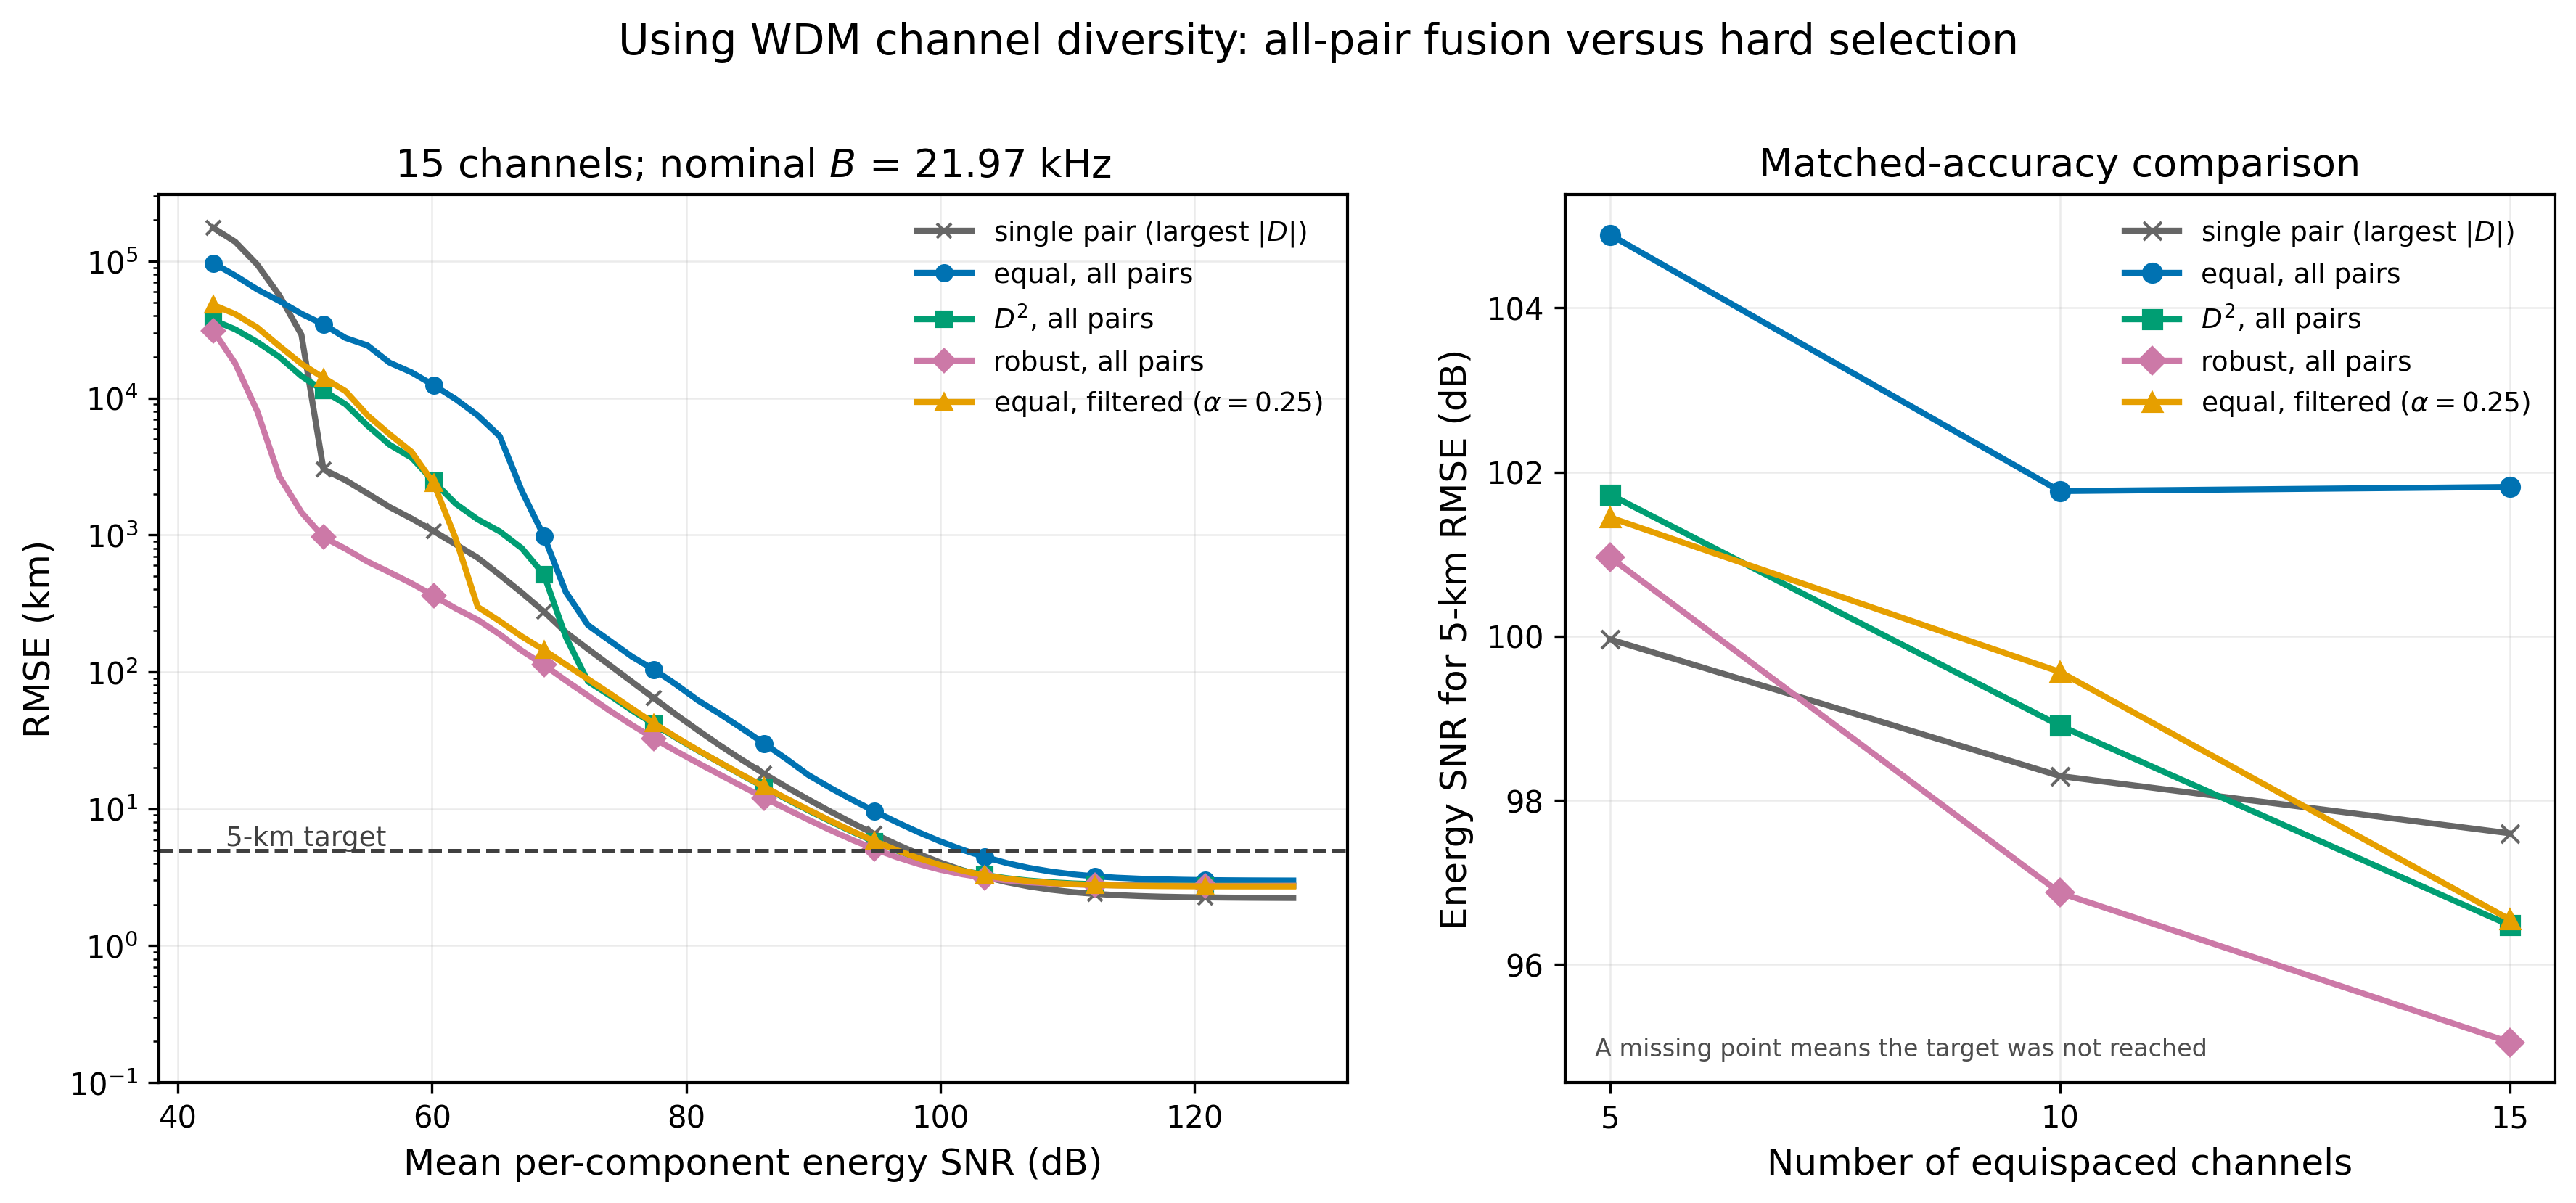
\includegraphics[width=\linewidth]{F10_equispaced_fusion_strategy.png}
\caption{Channel diversity and fusion on the equispaced parabolic run at
nominal $B\approx22$\,kHz. Left: 15-channel RMSE versus per-component energy
SNR for a single pair chosen by largest known $|D|$, equal fusion over all
pairs, all-pair $D^2$ and robust fusion, and equal fusion after the
$\alpha=0.25$ pair filter. Right: energy SNR required for RMSE $=5$\,km versus
channel count. Missing points mean the target was not reached in the saved SNR
sweep. These are empirical RMSE comparisons; pair estimates are correlated.}
\label{fig:strategy}
\end{figure}

The 15-channel, 22-kHz example in Fig.~\ref{fig:weights} explains what
``soft'' means here. At $\alpha=0.25$, the hard filter retains 32 of 105
equispaced pairs. Under all-pair $D^2$ weighting, pairs below that threshold
still carry about 26.2\% of the normalized sum of $D^2$ weights. That number is
the deterministic weight share, not a measured fraction of independent
Fisher information: the pair errors are correlated and can be biased. For this
15-channel subset, the saved $|D|$ values range from about 126 to 2129 ps/km,
so the dispersion quality is graded rather than split into just two groups.

\begin{figure}[t]
\centering
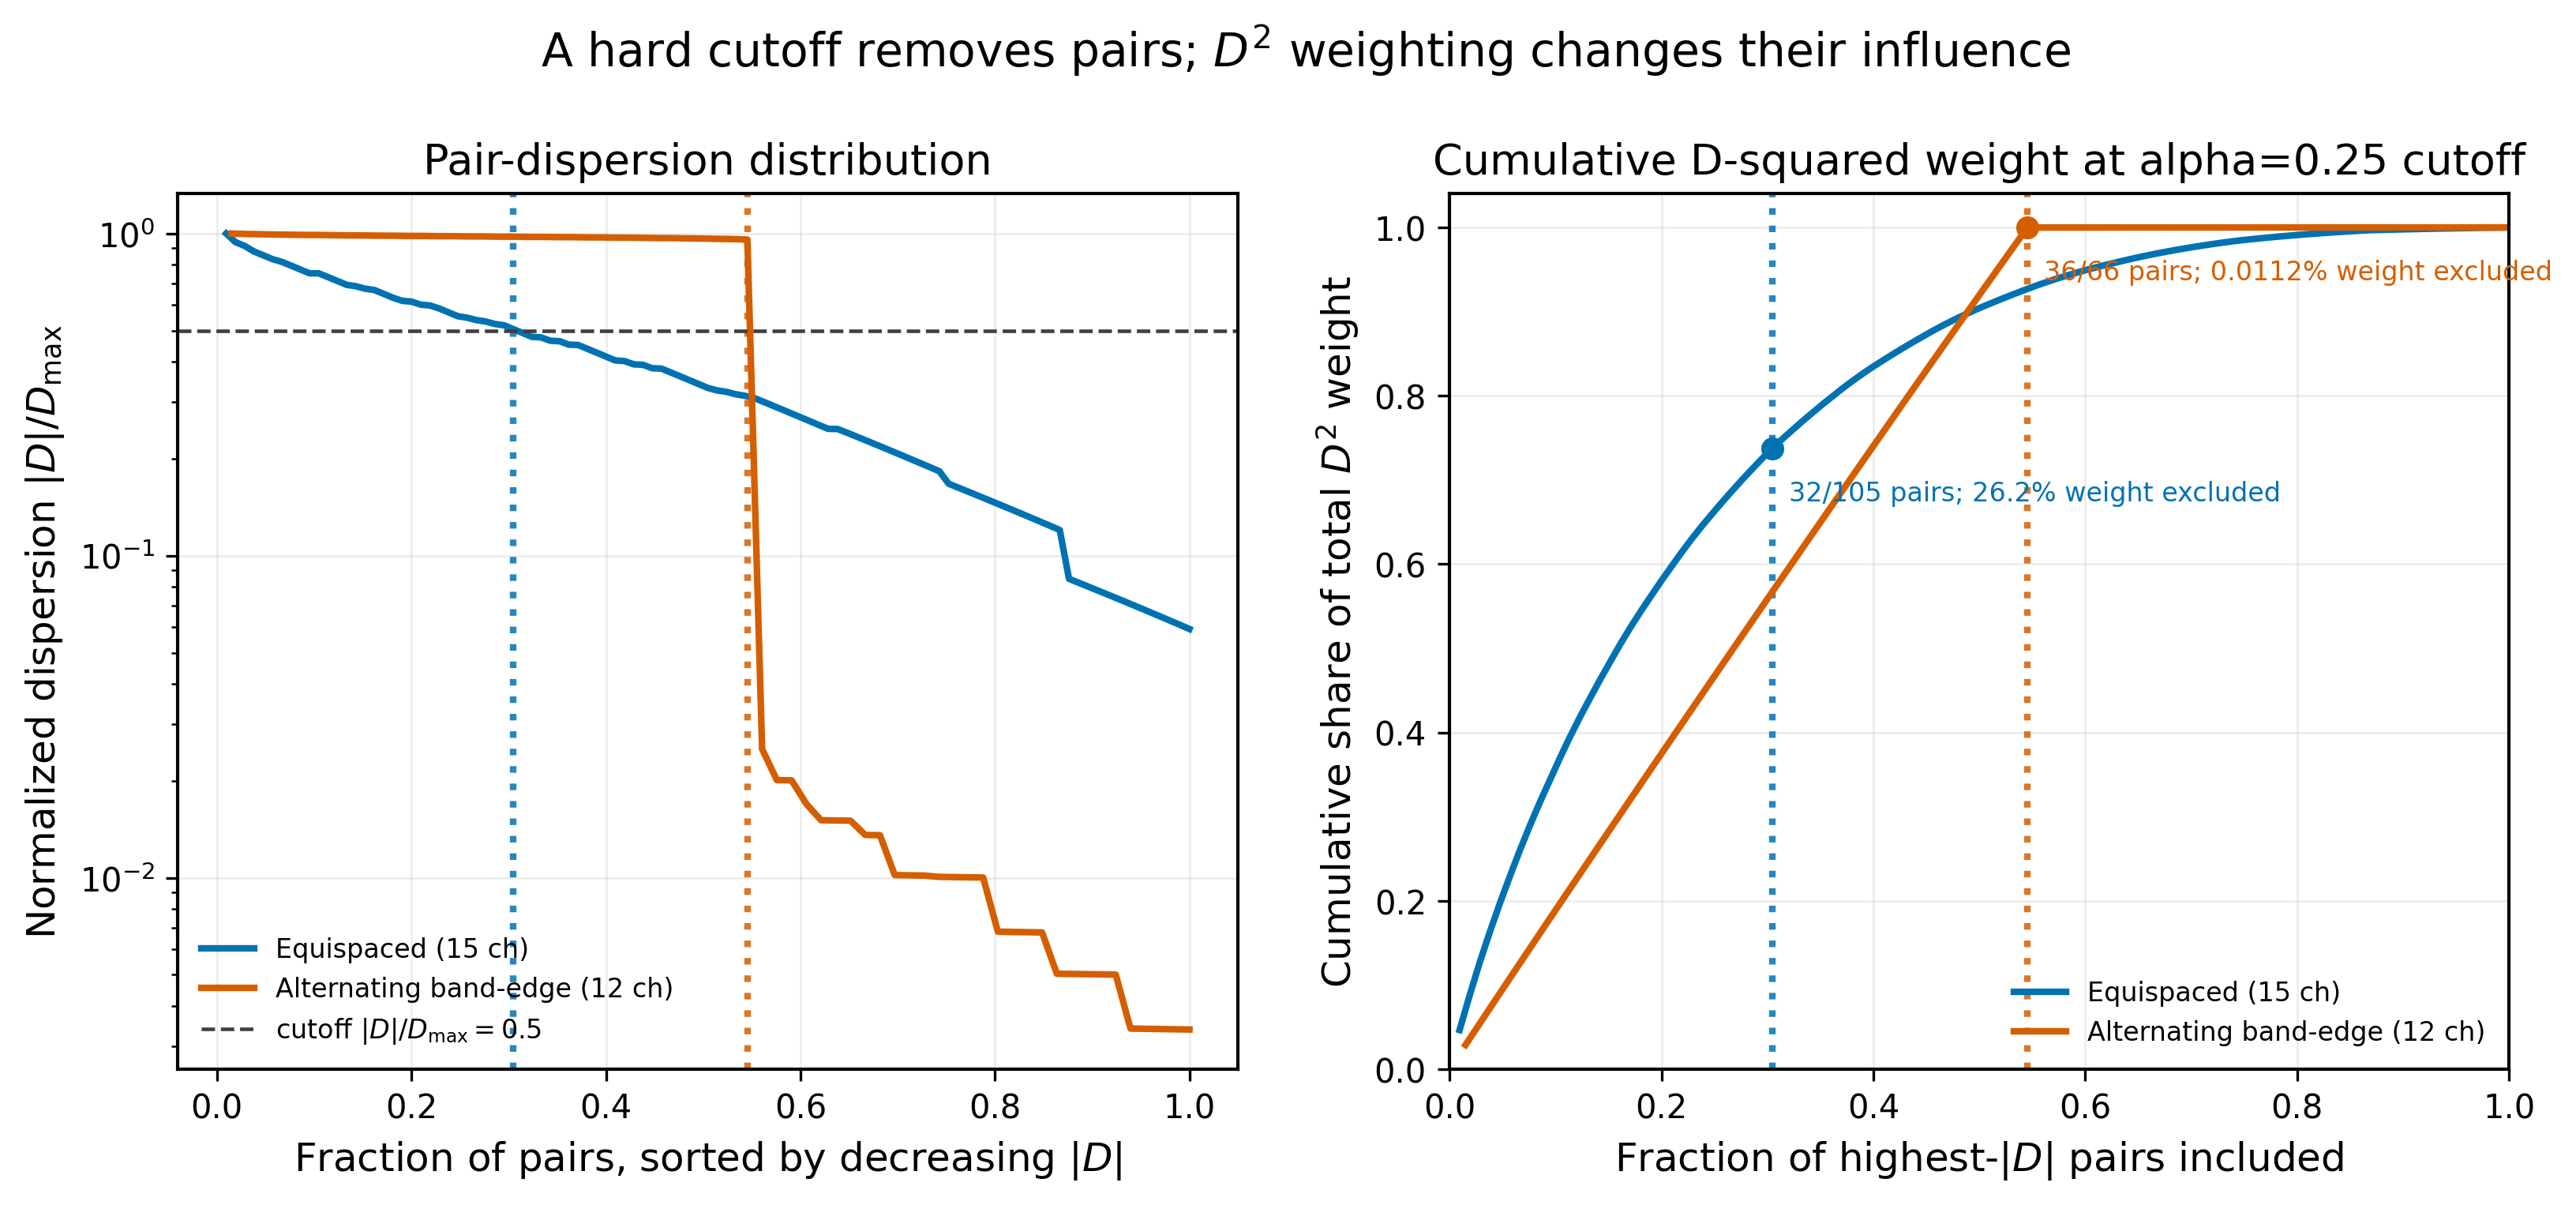
\includegraphics[width=0.96\linewidth]{F11_pair_weight_distribution.png}
\caption{Pair-dispersion and $D^2$-weight distributions for an equispaced
15-channel subset and the 12-channel alternating extremes-inward subset of the
241-channel master grid. At $\alpha=0.25$ (equivalently
$|D|/D_{\max}\ge0.5$), the equispaced filter retains 32/105 pairs; pairs below
the cutoff still hold 26.2\% of the all-pair $D^2$ weight. The band-edge filter
retains 36/66 pairs, while the excluded group holds only 0.011\% of the $D^2$
weight. This is weight allocation, not independent statistical information.}
\label{fig:weights}
\end{figure}

Figure~\ref{fig:alpha} is a different summary of the same parabolic,
equispaced study. For every $\alpha$, it compares the SNR needed for 5-km RMSE
with $D^2$ weights against the SNR needed with equal weights on the
\emph{same} selected pair pool, then averages the finite savings over the
bandwidth sweep. A positive ordinate means $D^2$ needs less SNR; zero means a
tie. At $\alpha=0$ (all pairs), the mean savings are about 3.6\,dB for 5
channels, 2.9\,dB for 10, and 4.8\,dB for 15. As $\alpha$ grows, the added
weighting gain generally shrinks: the hard cutoff has already removed many
low-dispersion pairs, so there is less for continuous weighting to improve.
The plotted sweep does not contain exactly $\alpha=0.25$; that default lies
between the displayed 0.20 and 0.30 cases.

\begin{figure}[t]
\centering
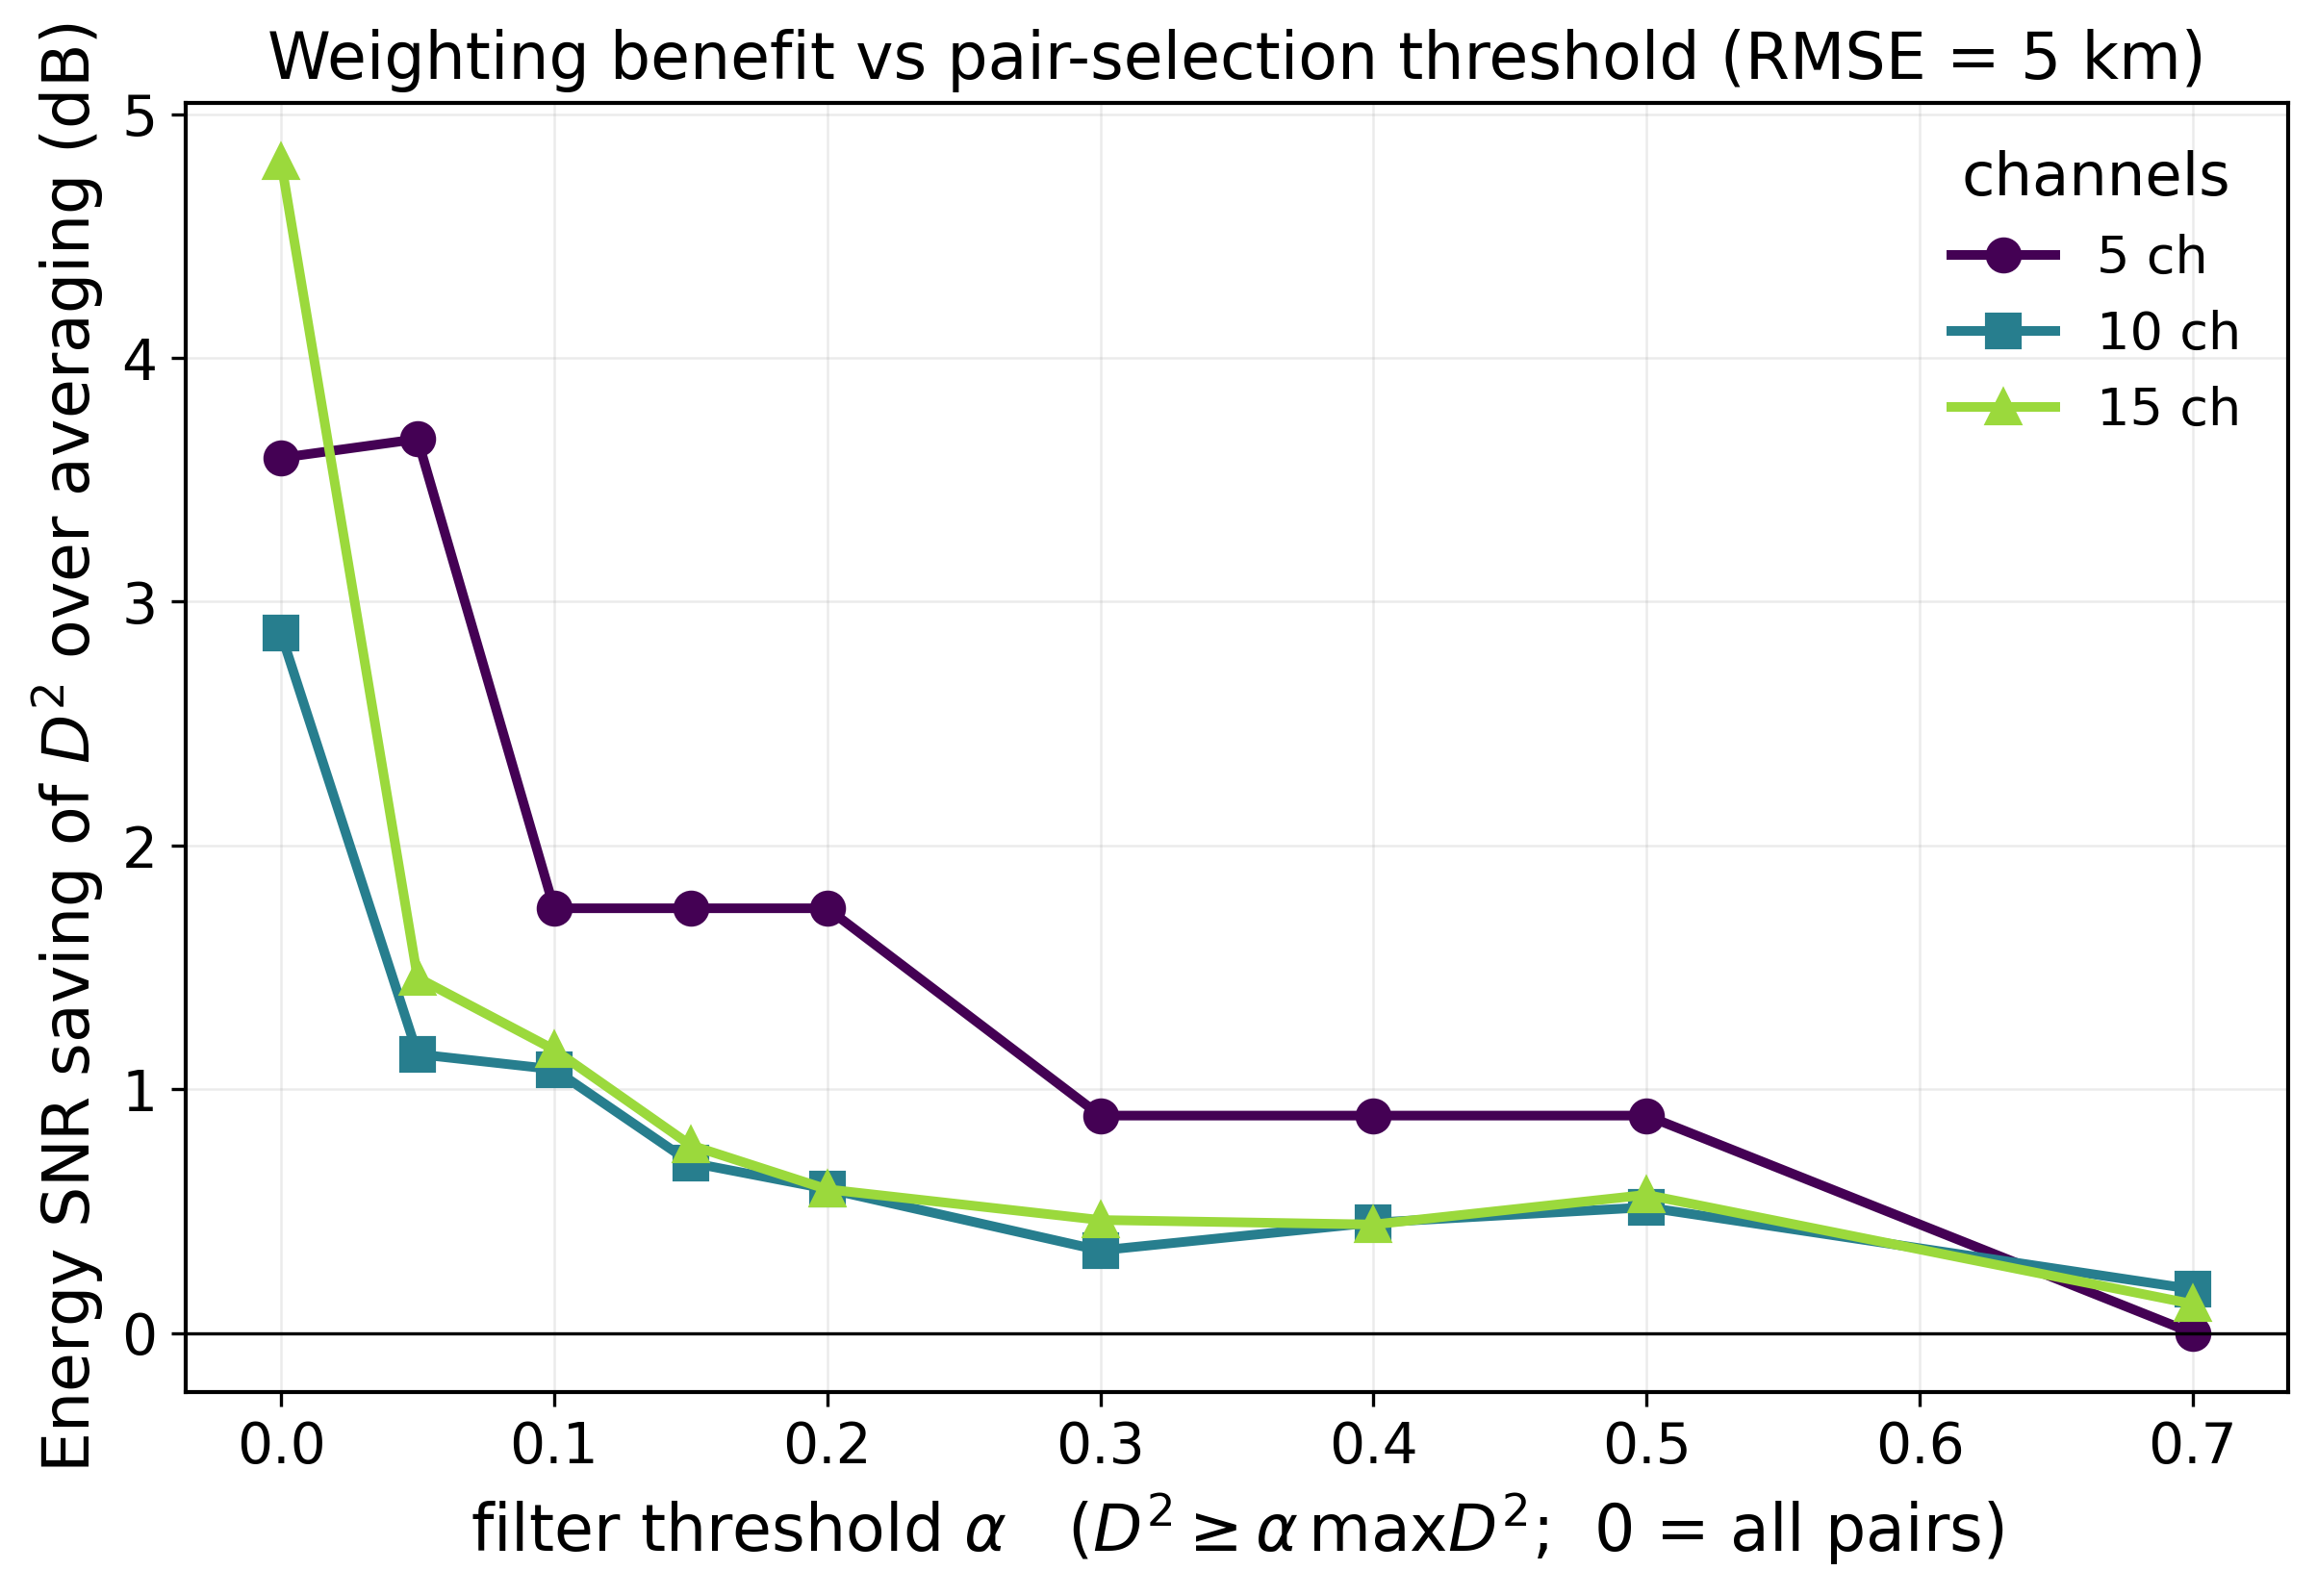
\includegraphics[width=0.9\linewidth]{F8_alpha_sweep.png}
\caption{Weighting benefit versus filter threshold $\alpha$
($(D^{\rm abs})^2\ge\alpha\max(D^{\rm abs})^2$; $\alpha=0$ means all pairs),
per channel count, on the equispaced parabolic run. The ordinate is the
energy-SNR saving of $D^2$ weighting over equal averaging on the same pool at
RMSE $=5$\,km, averaged over bandwidth values. Positive values favor $D^2$; the
general decrease with $\alpha$ shows that selection leaves less incremental
benefit for weighting.}
\label{fig:alpha}
\end{figure}

\subsection{Why the alternating band-edge grid behaves differently}
The band-edge configuration is an alternating extremes-inward selection from
the 241-channel, 50-GHz master grid. For 12 selected channels it places six
carriers at each spectral edge. This produces 30 within-edge pairs with small
dispersion and 36 cross-edge pairs with much larger dispersion. As a result,
the pair-dispersion distribution is nearly separated into low- and high-$|D|$
groups rather than varying gradually: the saved within-edge values range from
about 7 to 55 ps/km, while cross-edge values range from about 2099 to
2191 ps/km. The target-SNR crossings are tabulated in Table~\ref{tab:bandedge_snr}.

\begin{table}[t]
\centering
\caption{Energy SNR (dB) required for 5-km RMSE on the alternating band-edge
parabolic run near nominal $B=22.51$\,kHz. The filtered-equal pool uses
$\alpha=0.25$.}
\begin{tabular}{rcccc}
\toprule
Channels & Equal, all pairs & $D^2$, all pairs & Robust, all pairs & Equal, filtered \\
\midrule
6  & 127.38 & 92.91 & 92.92 & 92.91 \\
8  & 124.39 & 91.57 & 91.57 & 91.57 \\
10 & 122.39 & 90.38 & 90.38 & 90.38 \\
12 & 119.84 & 90.02 & 90.02 & 90.01 \\
\bottomrule
\end{tabular}
\label{tab:bandedge_snr}
\end{table}

At 6--12 channels, explicit filtering saves about 30--34\,dB relative to
equal averaging over all pairs. Yet all-pair $D^2$ and robust estimates reach
the 5-km target at almost the same SNR as filtered equal averaging. For 12
channels, the 30 pairs below the $\alpha=0.25$ threshold have only 0.011\% of
the total all-pair $D^2$ weight. Thus the weighted estimate has not literally
deleted them, but their aggregate influence is negligible. This is why the
band-edge case is a contrast, not the main demonstration that soft weighting
retains lower-dispersion contributions.

\begin{figure}[t]
\centering
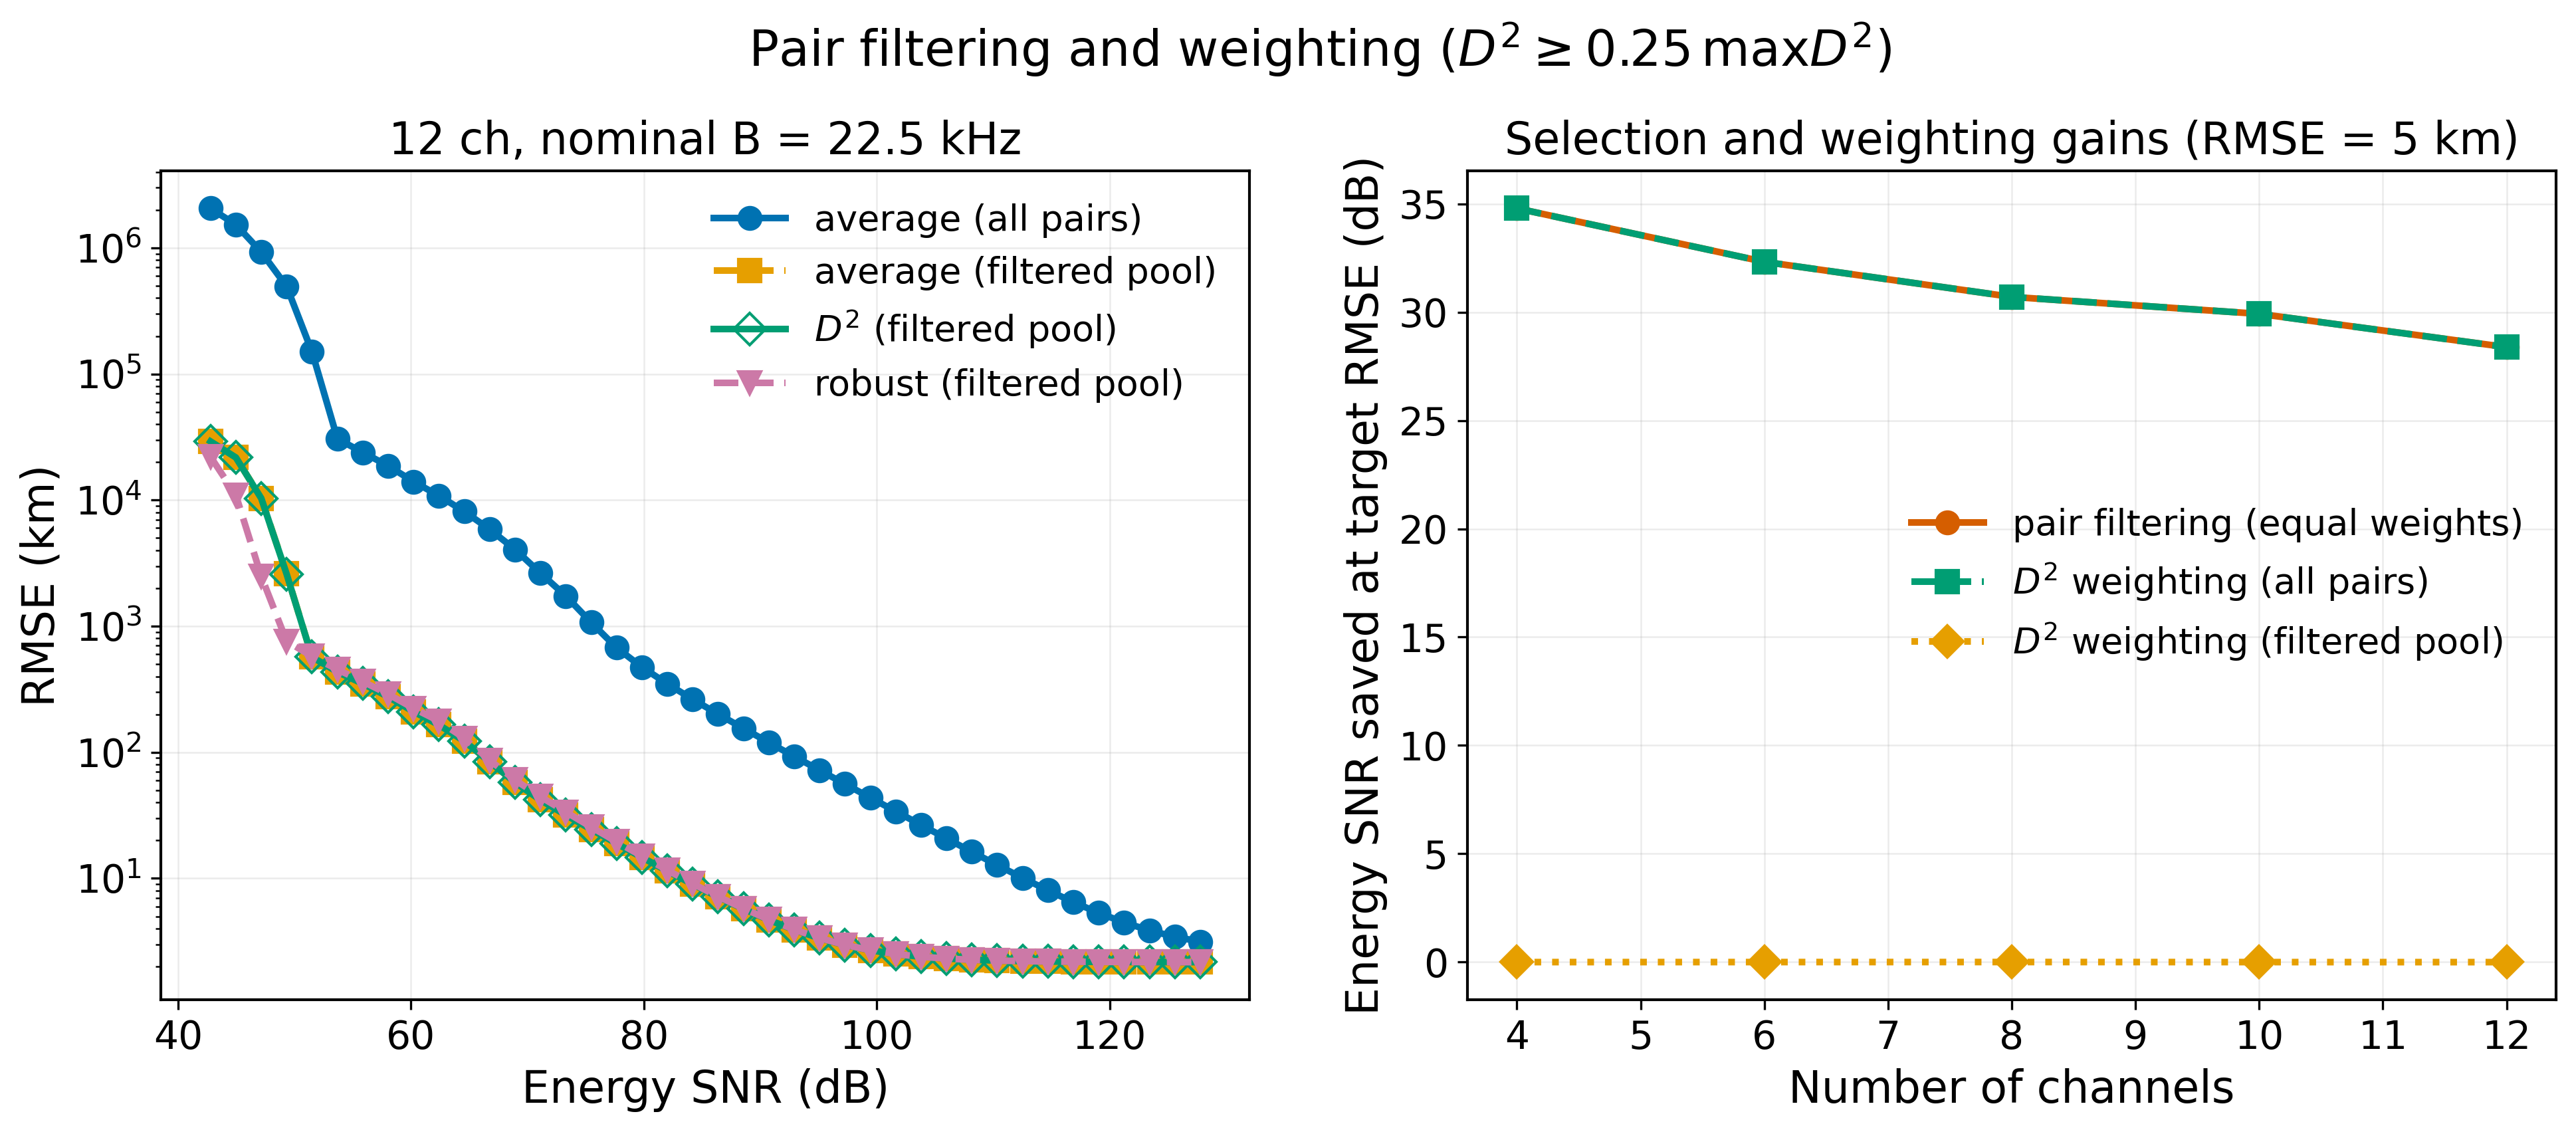
\includegraphics[width=\linewidth]{bandedge_pair_filtering.png}
\caption{Pair filtering on the parabolic run with 12 channels selected
alternating extremes-inward from the 50-GHz master grid (nominal
$B\approx22.5$\,kHz). The left panel compares equal weighting over all pairs
with equal, $D^2$, and robust fusion on the filtered pool
[$(D^{\rm abs})^2\ge0.25\max(D^{\rm abs})^2$]. The right panel separates the
energy-SNR saving due to filtering from the additional gain due to $D^2$
weighting. The plotted RMSE includes estimator bias; no combined-CRB
attainment is claimed.}
\label{fig:bandedge}
\end{figure}

\subsection{Robust fusion in the GCC-PHAT regime}
Figures~\ref{fig:pool}, \ref{fig:biasvar}, and~\ref{fig:ecdf} use the
equispaced GCC-PHAT run, whereas Fig.~\ref{fig:strategy} and the $D^2$
threshold sweep use parabolic estimates. Their magnitudes should not be
compared as if only the fusion rule changed. In Fig.~\ref{fig:pool}, the left
panel fixes 15 channels and nominal $B\approx22$\,kHz and compares equal
averaging over all pairs with equal, $D^2$, and robust fusion on the
$\alpha=0.25$ filtered pool. The right panel is not the same single-bandwidth
comparison: it averages target-SNR savings over bandwidth cells for each
channel count.

At 15 channels and nominal $B=21.97$\,kHz, the saved GCC-PHAT metrics at the
largest tested energy SNR, $127.78$\,dB, are striking. In the filtered pool,
equal averaging has RMSE $345.18$\,km, $D^2$ weighting has $231.58$\,km, and
robust fusion has $0.712$\,km. Robust fusion reaches 5-km RMSE at about
$99.57$\,dB, while filtered equal and filtered $D^2$ do not cross 5\,km
anywhere in the tested SNR range. These are results for this particular
GCC-PHAT cell, not a universal guarantee.

The algorithmic reason the curves can separate is that $D^2$ weights depend
only on known dispersion. They cannot recognize a pair whose GCC-PHAT peak is
bad for the current realization. Robust fusion adds the Tukey residual factor
of Eq.~\eqref{eq:robustweights}; it preserves estimates near the cross-pair
consensus and suppresses remote ones. The saved data are consistent with
strong pair-specific outliers and bias in this cell. F6 decomposes RMSE into
spread and bias; at the highest SNR, the filtered-pool robust estimate has
bias $-0.684$\,km and standard deviation $0.197$\,km, while filtered equal and
$D^2$ have biases $-91.37$\,km and $-61.87$\,km, respectively. Robust fusion
is therefore addressing more than ordinary variance differences. Because it
uses the observed pair estimates to form weights, it can also fail when the
majority consensus is itself wrong; its advantage must be established
empirically for each estimator and operating regime.

In the 15-channel GCC-PHAT design curve (Fig.~\ref{fig:design}), the filtered
equal and filtered $D^2$ curves have no final 15-channel point because neither
method reaches 5-km RMSE before the maximum tested SNR. This is intentional,
not missing data. The robust filtered-pool curve does reach the target. At the
selected ECDF cell, nominal $B\approx22$\,kHz and energy SNR $77.48$\,dB,
robust filtered-pool fusion also has a much lighter error tail: its RMSE is $63.6$\,km,
versus $7.19\times10^3$\,km for filtered equal and $6.53\times10^3$\,km for
filtered $D^2$. The ECDF in Fig.~\ref{fig:ecdf} plots the fraction of estimates
with $|e|\le x$; a curve farther left and higher is better. Its vertical 1\%
and 5\% lines correspond to 5 and 25\,km because the true range is 500\,km.
It is a single operating-cell tail comparison, not a sweep-wide guarantee.

\begin{figure}[t]
\centering
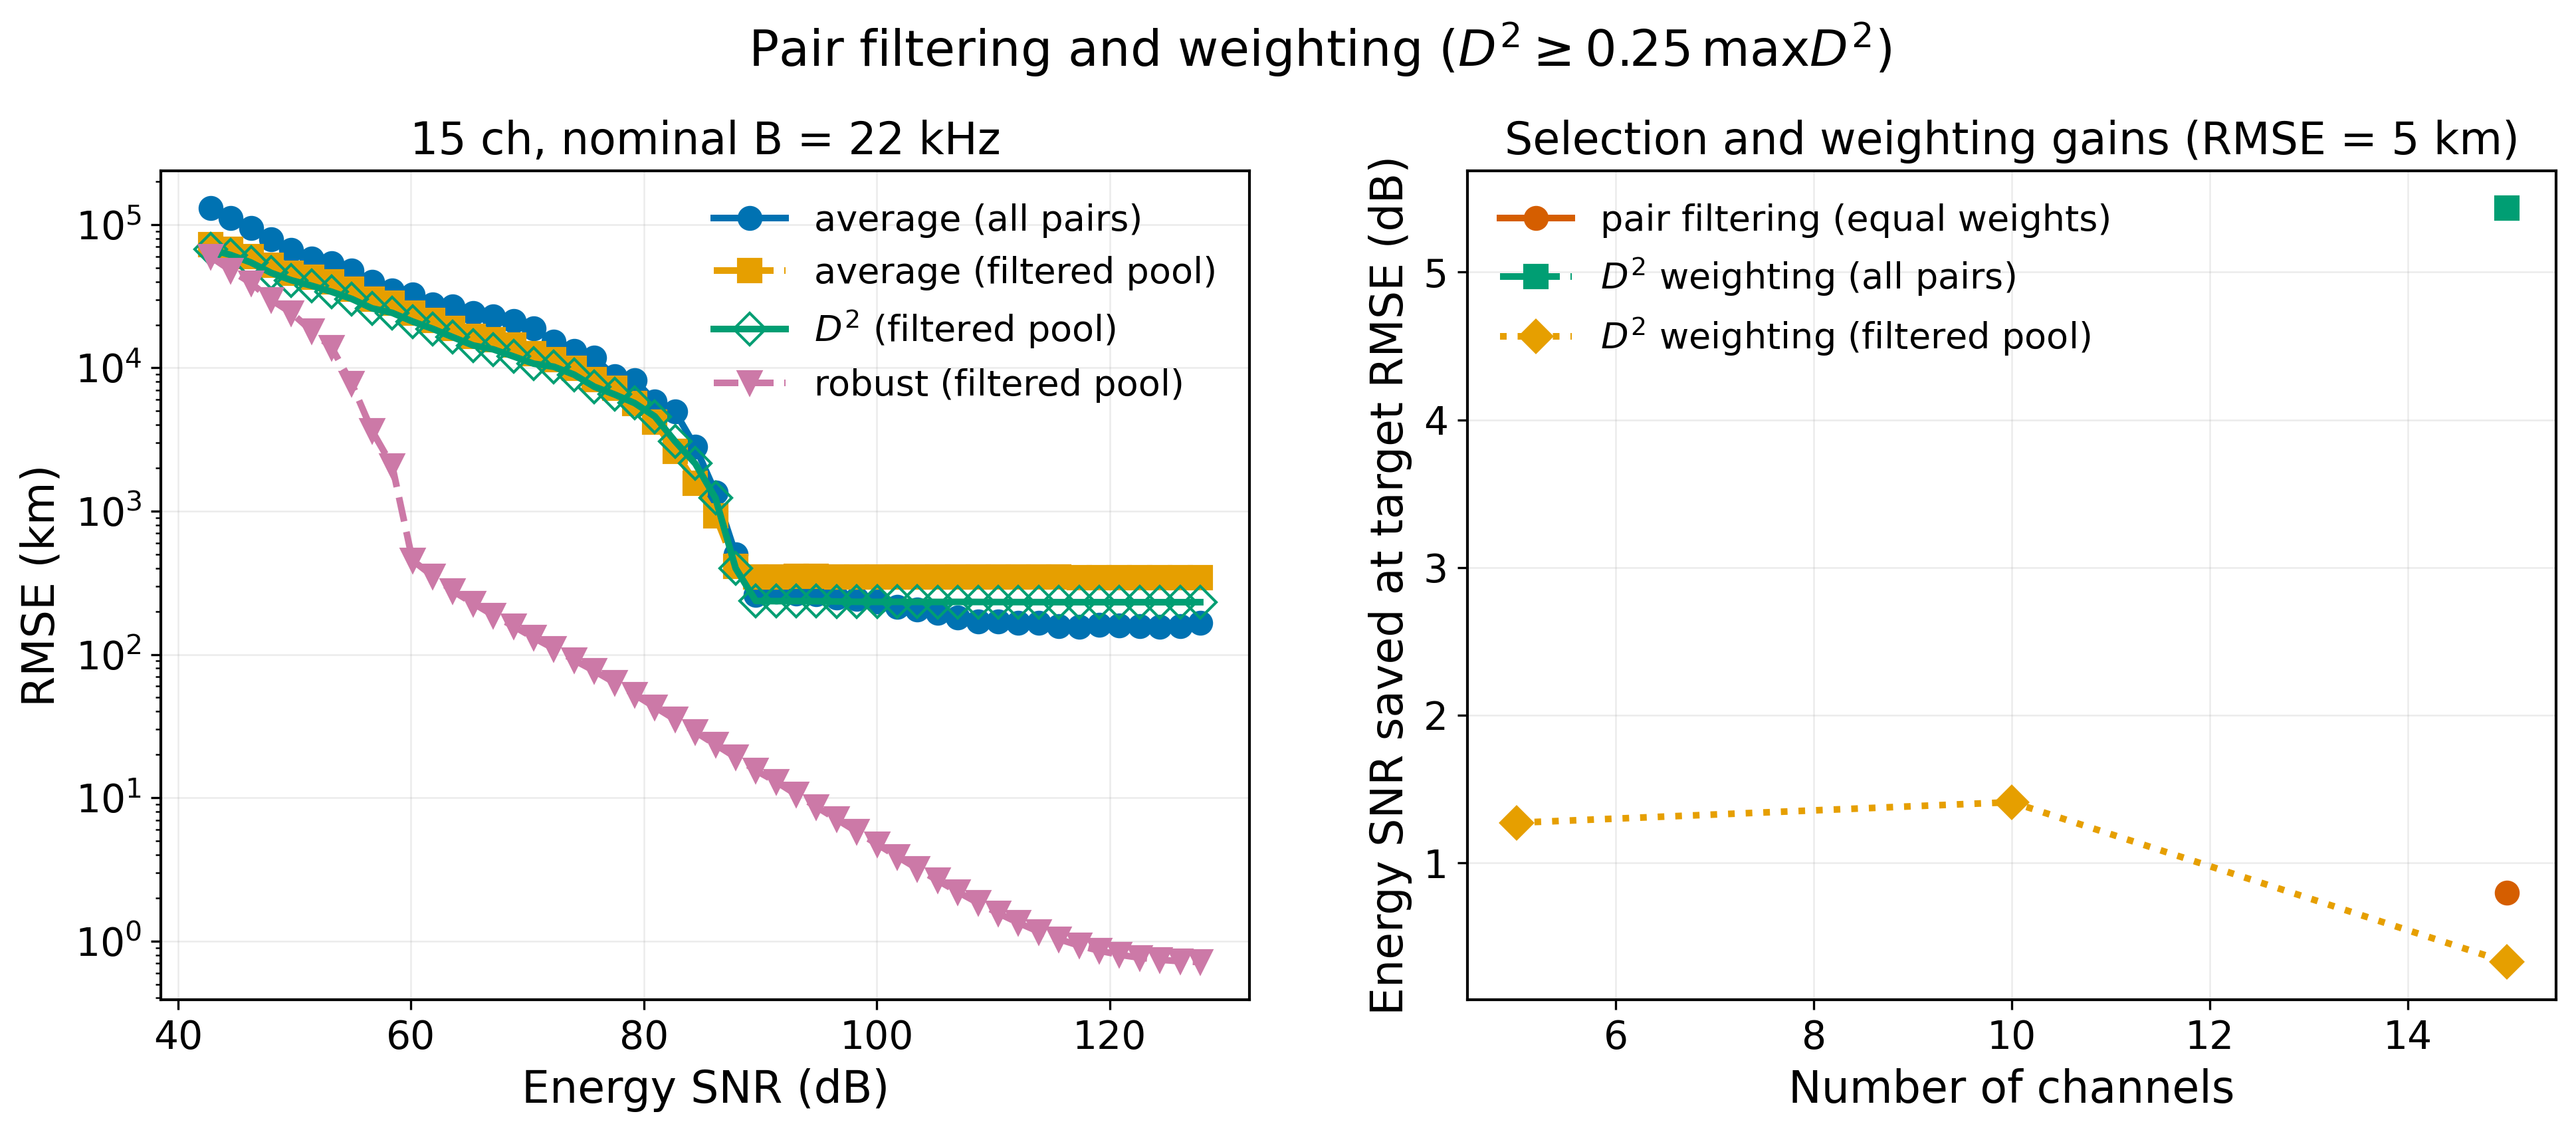
\includegraphics[width=\linewidth]{F7_pool_effect.png}
\caption{Pair filtering and weighting on the 15-channel equispaced GCC-PHAT
run (nominal $B\approx22$\,kHz). Left: RMSE for equal weighting over all pairs
and for equal, $D^2$-weighted, and robust fusion on the filtered pool
[$(D^{\rm abs})^2\ge0.25\max(D^{\rm abs})^2$]. Right: energy-SNR savings at
RMSE $=5$\,km from filtering with equal weights and from $D^2$ weighting on
all pairs or on the filtered pool, averaged over bandwidth cells where both
target crossings are defined. Robust is shown for the filtered pool in the
left panel. These are empirical comparisons, not a combined-CRB plot.}
\label{fig:pool}
\end{figure}

\subsection{Estimator bias and the meaning of RMSE}
Figure~\ref{fig:estimators} compares parabolic and GCC-PHAT pair estimation
after the same robust fusion rule at 15 channels. It shows a crossover, not a
universal SNR threshold: parabolic interpolation often has lower variance at
low SNR, while the reduced peak-shape bias of GCC-PHAT can make it preferable
at high SNR or high nominal bandwidth. ``GCC-PHAT only works at high SNR'' is
too broad; the result depends jointly on SNR, $B_{\rm nom}$, PMD-induced peak
shape, and the chosen fusion.

Figure~\ref{fig:biasvar} makes the high-SNR error floor explicit. The left
panel plots RMSE and standard deviation; the right plots absolute bias. When
noise becomes small, standard deviation can continue to decrease while RMSE
stops improving because the bias remains. For the robust GCC-PHAT pool near
22\,kHz the high-SNR bias is about $-0.68$\,km. At the same cell the
parabolic bias is about $-2.63$\,km. At nominal $B=2$\,MHz the GCC-PHAT bias is
close to zero in the tested run. Table~\ref{tab:est} gives representative
RMSE values: at 22\,kHz and 127.8\,dB, GCC-PHAT RMSE is approximately 0.71\,km
for 15 channels versus 2.64\,km for parabolic; at 1.3\,kHz and 103.8\,dB,
parabolic is better (25.8\,km versus 52.3\,km for GCC-PHAT). This is why the
paper reports both bias and spread instead of presenting a single variance
curve as accuracy.

\begin{table}[t]
\centering
\caption{RMSE (km) after robust fusion at representative envelope bandwidths
and energy SNRs. $B$ is the nominal Gaussian-envelope parameter.}
\begin{tabular}{lccccc}
\toprule
& \multicolumn{2}{c}{22\,kHz, 127.8\,dB} & \multicolumn{2}{c}{1.3\,kHz, 103.8\,dB} & 2\,MHz, 127.8\,dB\\
\cmidrule(lr){2-3}\cmidrule(lr){4-5}\cmidrule(lr){6-6}
Channels & Parabolic & GCC-PHAT & Parabolic & GCC-PHAT & Parabolic / GCC-PHAT\\
\midrule
10 & 2.65 & \textbf{0.73} & \textbf{30.5} & 61.8 & 0.035 / \textbf{0.006}\\
15 & 2.64 & \textbf{0.71} & \textbf{25.8} & 52.3 & 0.035 / \textbf{0.004}\\
\bottomrule
\end{tabular}
\label{tab:est}
\end{table}

\begin{figure}[t]
\centering
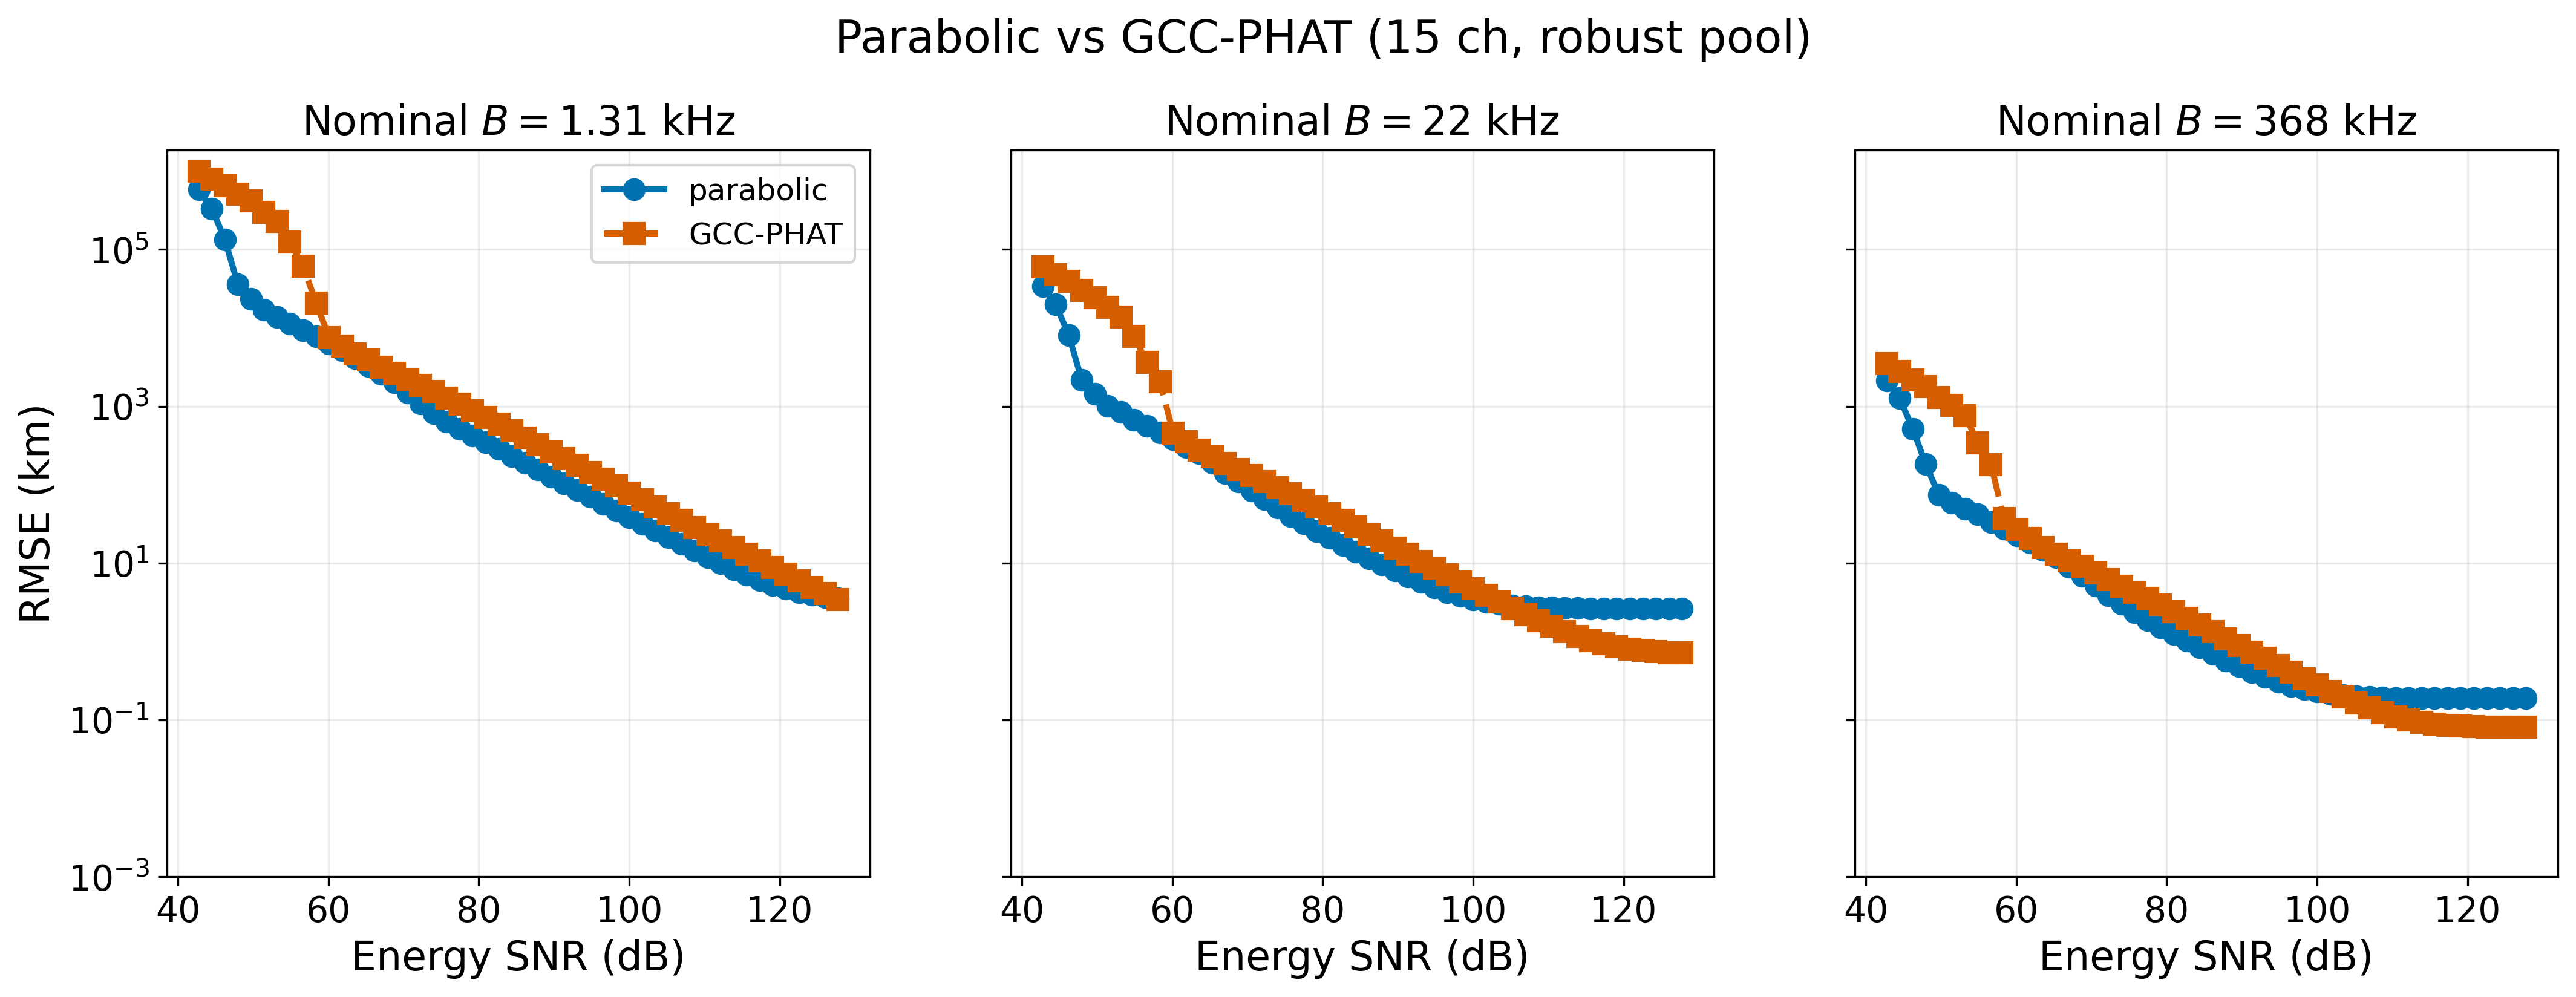
\includegraphics[width=0.95\linewidth]{F1_estimators_compare.png}
\caption{RMSE versus per-component energy SNR at three nominal envelope
parameters (15 channels, $\alpha=0.25$ filtered pool) for parabolic and
GCC-PHAT delay estimation. The estimators cross: parabolic often has lower
RMSE at lower SNR, while GCC-PHAT can reduce the high-SNR bias floor. The
crossover is bandwidth-dependent, not a universal SNR threshold.}
\label{fig:estimators}
\end{figure}

\subsection{A secondary covariance-aware fusion benchmark}
Figure~\ref{fig:covgls} asks whether learning the full empirical covariance
among pair errors gives a measurable improvement over the simpler rules. For
each SNR at the selected bandwidth, half the realizations train the covariance
weights and the other half evaluate them. The figure shows held-out RMSE,
standard deviation, and absolute bias. At high SNR the curves are very close:
all filtered estimators have roughly $0.1$\,km standard deviation and about
$2.6$\,km absolute bias, so the shared bias dominates RMSE. For this split,
empirical-covariance GLS has RMSE $2.65$\,km, standard deviation $0.097$\,km,
and bias $-2.65$\,km; robust filtered fusion has RMSE $2.63$\,km, standard
deviation $0.107$\,km, and bias $-2.63$\,km. The benchmark's value is
methodological: it tests a covariance-aware alternative without calling it a
bound, and shows little extra gain in this particular bias-limited cell. It is
secondary to the main WDM-diversity result.

\begin{figure}[t]
\centering
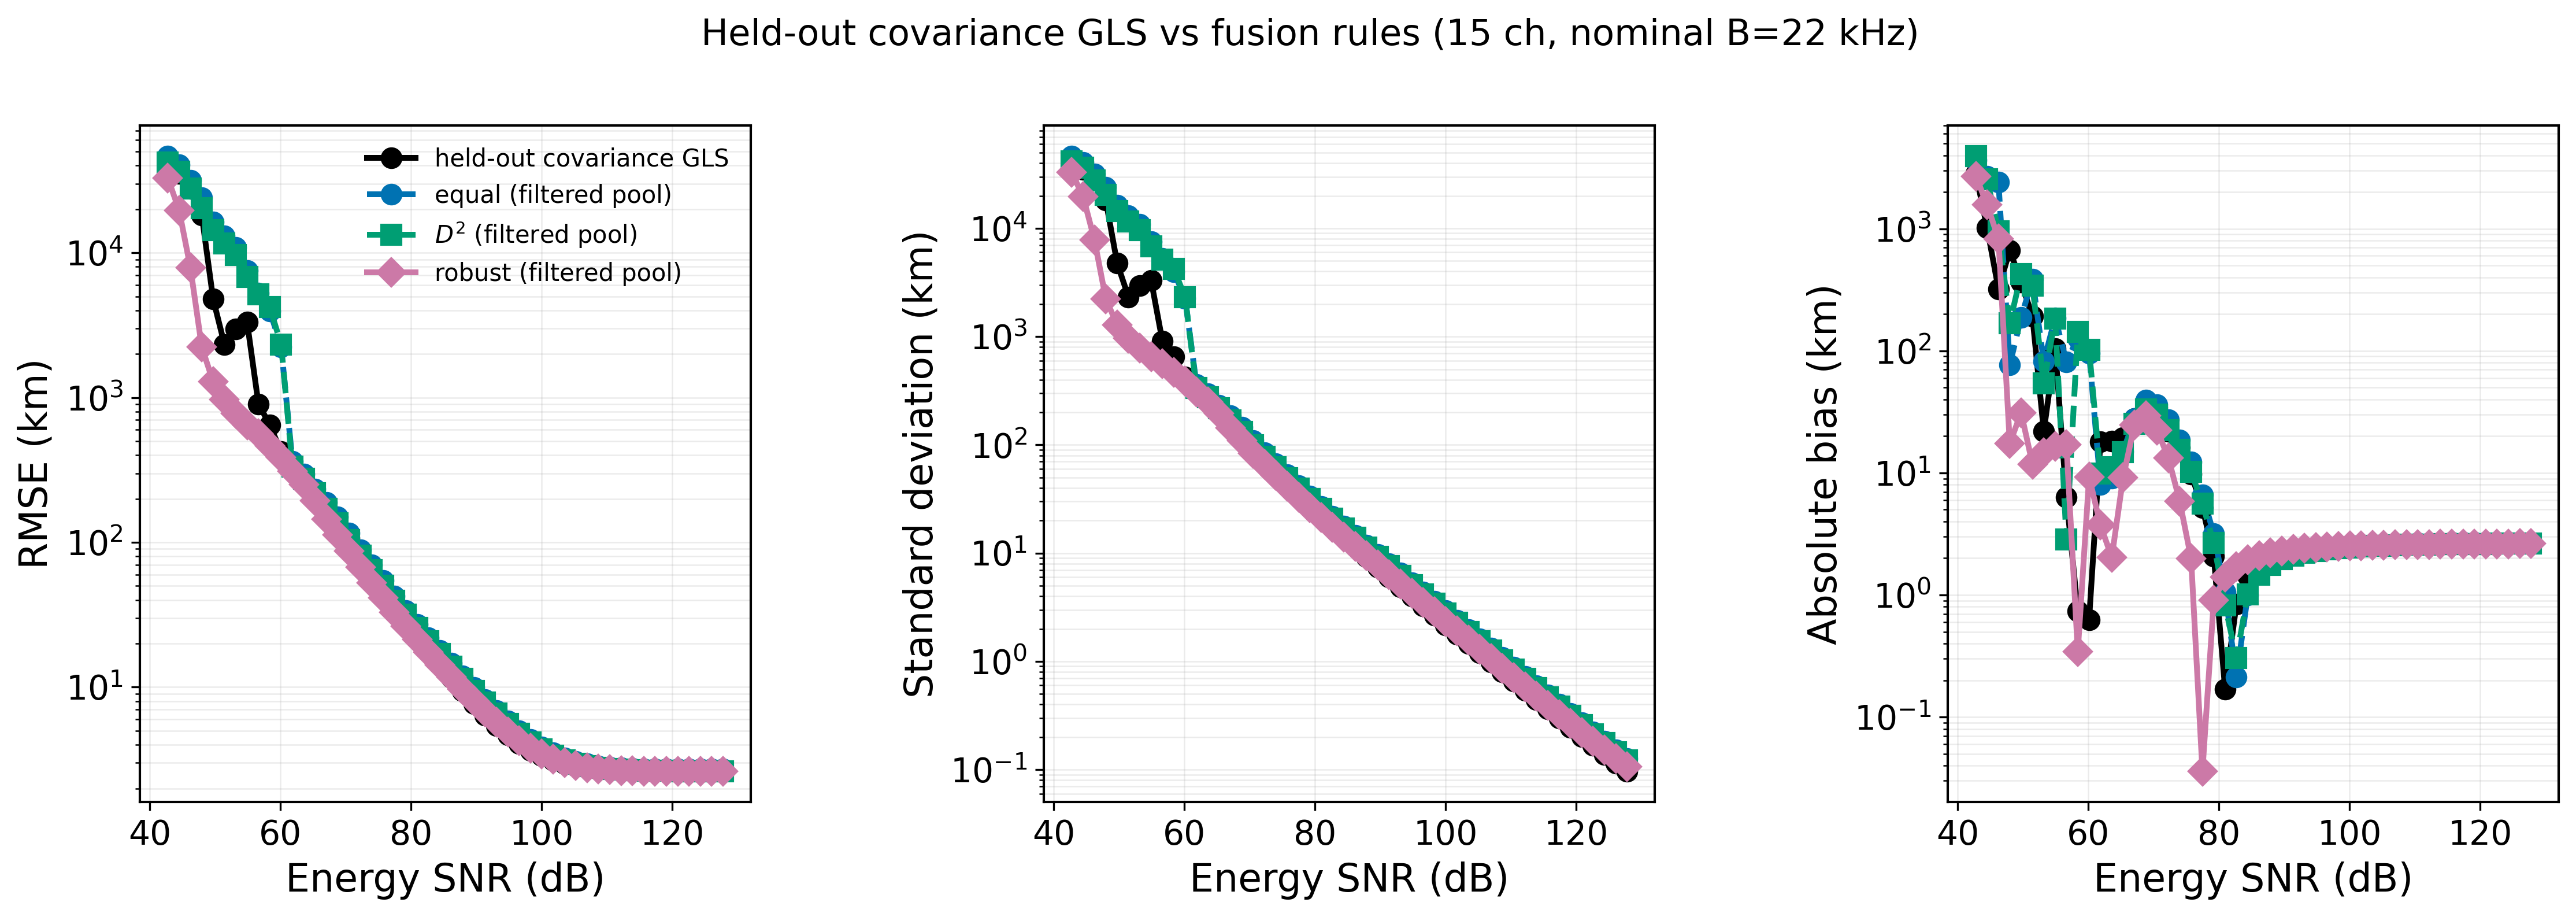
\includegraphics[width=\linewidth]{F9_empirical_covariance_gls.png}
\caption{Held-out empirical-covariance GLS benchmark versus fusion rules
(15-channel equispaced parabolic run, nominal $B\approx22$\,kHz). At each SNR,
pair-error covariance is estimated from even-indexed realizations with 5\%
diagonal shrinkage; the covariance GLS uses all pairs, while equal, $D^2$, and
robust comparison curves use the $\alpha=0.25$ filtered pool. Curves are
evaluated on odd-indexed realizations. Similar high-SNR curves indicate little
extra covariance-weighting gain in this bias-limited cell, not equivalence in
all regimes. This is an empirical benchmark, not a CRB.}
\label{fig:covgls}
\end{figure}

\subsection{Bandwidth, SNR, channel count, and fibres}
In the tested high-SNR regime, the measured standard-deviation scale is
approximately
\begin{equation}
\sigma_Z\propto\frac{1}{\sqrt{\SNR_E}\,B_{\rm nom}},
\label{eq:scaling}
\end{equation}
consistent with a delay-information term proportional to SNR times squared
RMS bandwidth. This is an empirical scaling over the simulated range, not an
exact law at low SNR or in bias-dominated cells. Figure~\ref{fig:design}
provides a target-accuracy design view for GCC-PHAT. More channels often lower
the target SNR, but the curves can stop when an estimator's bias floor exceeds
the target. Averaging independent fibre realizations gives approximately
$1/\sqrt{N_{\rm fib}}$ spread reduction in the tested regime; it does not
remove a shared estimator bias.

\begin{figure}[t]
\centering
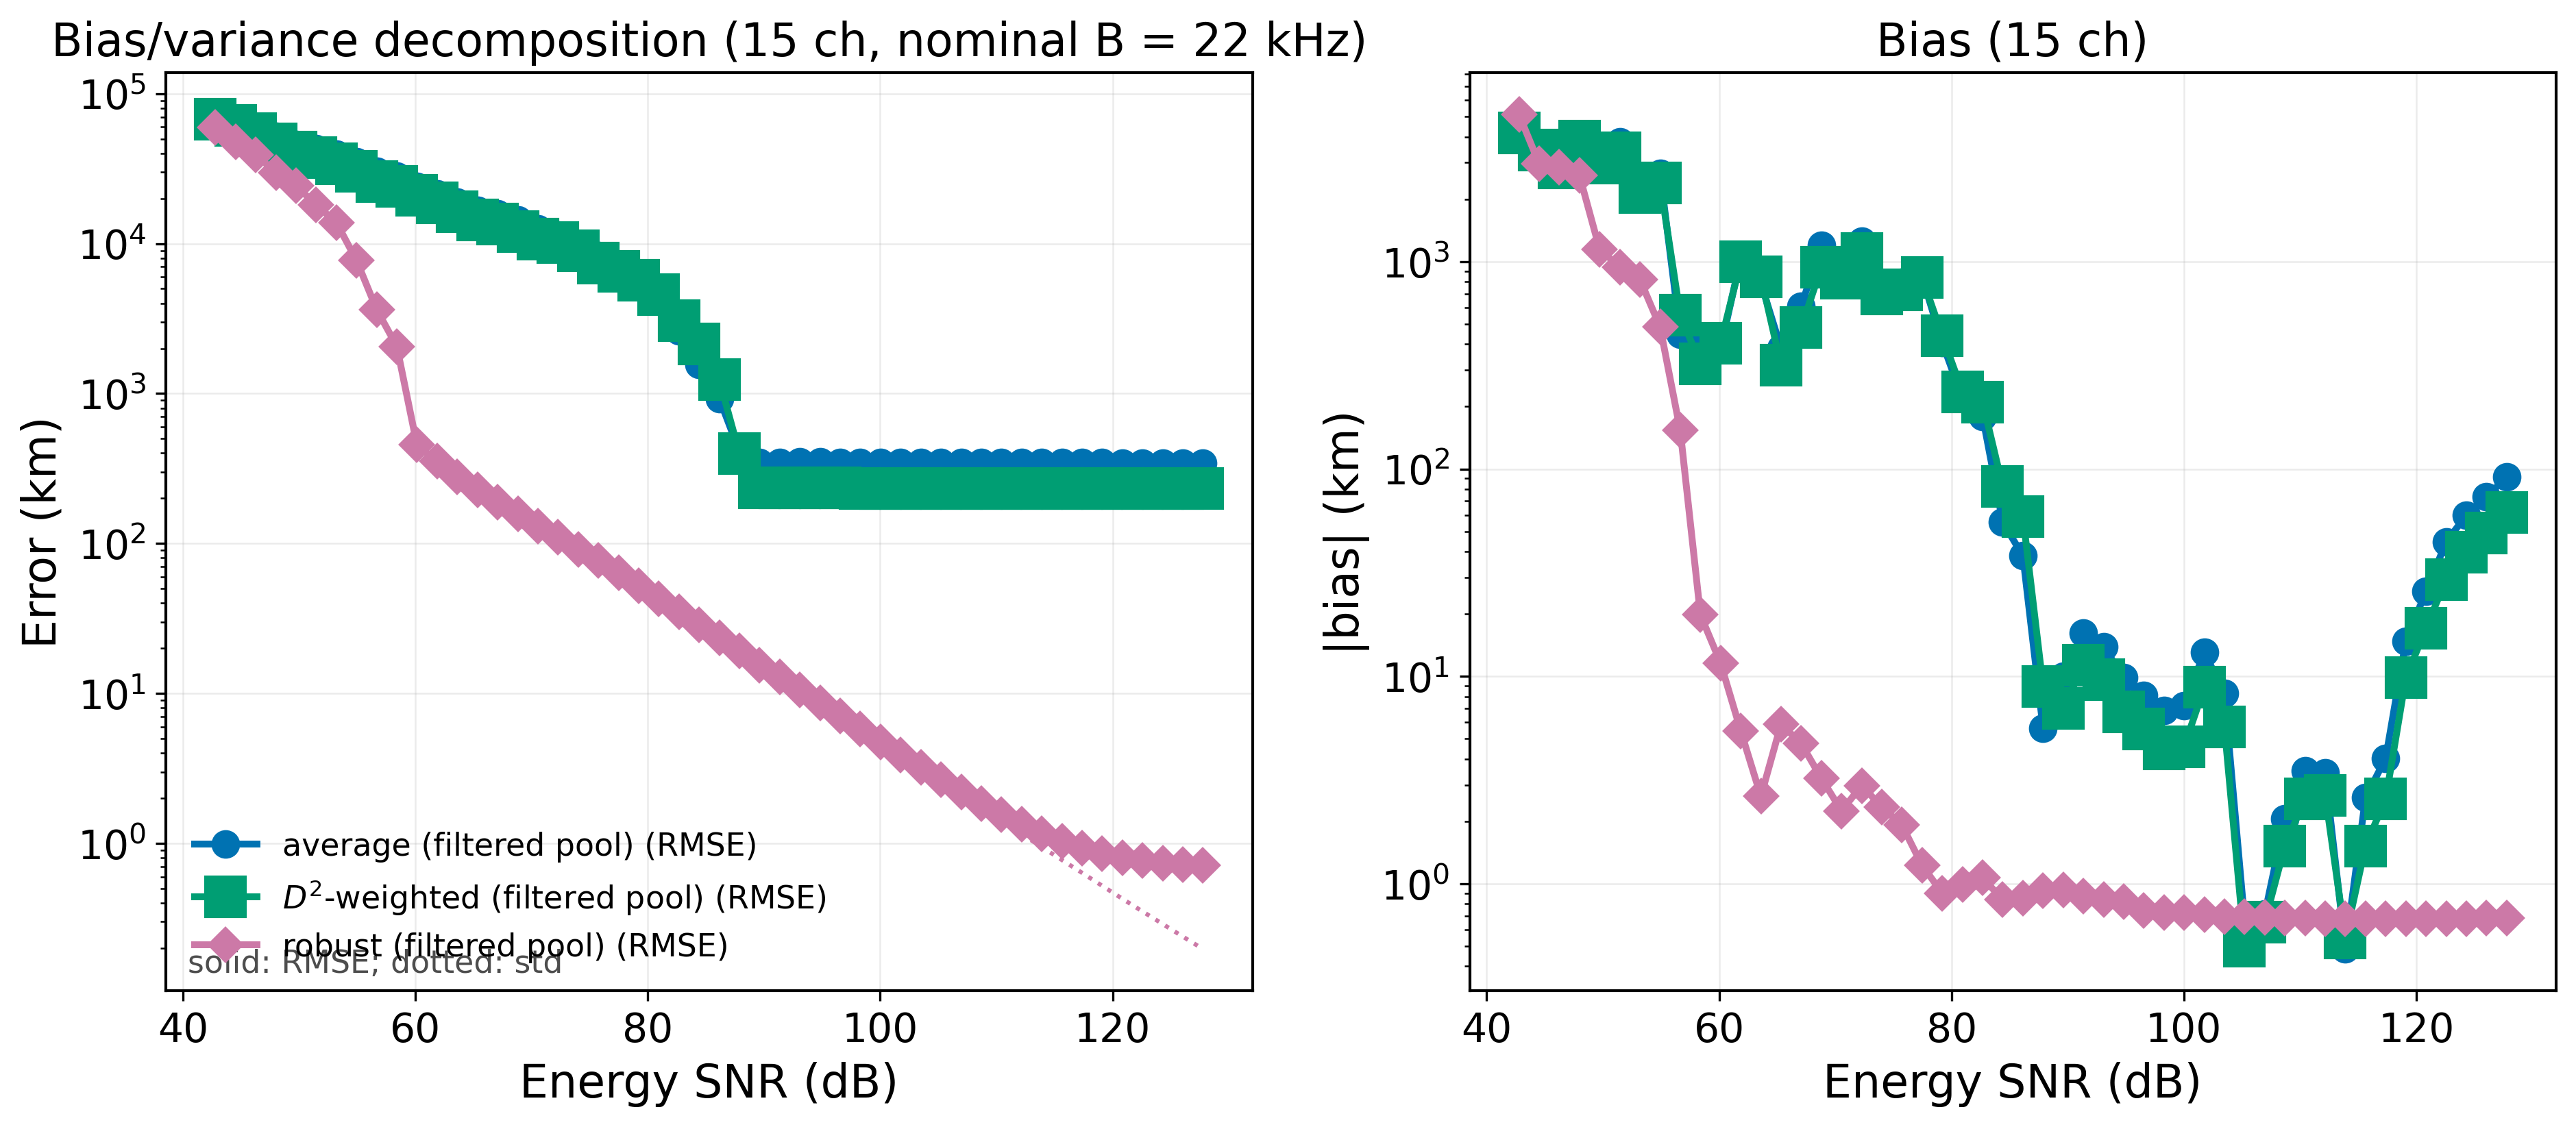
\includegraphics[width=\linewidth]{F6_bias_variance.png}
\caption{Bias/variance decomposition for the 15-channel equispaced GCC-PHAT
run at nominal $B\approx22$\,kHz, using the $\alpha=0.25$ filtered pool. Left:
RMSE (solid) and standard deviation (dotted) in km; right: absolute bias.
Non-robust filtered fusion has a severe high-SNR error floor in this cell,
whereas the residual-based robust rule suppresses the large pair deviations.
The remaining robust RMSE floor is bias-dominated.}
\label{fig:biasvar}
\end{figure}

\begin{figure}[t]
\centering
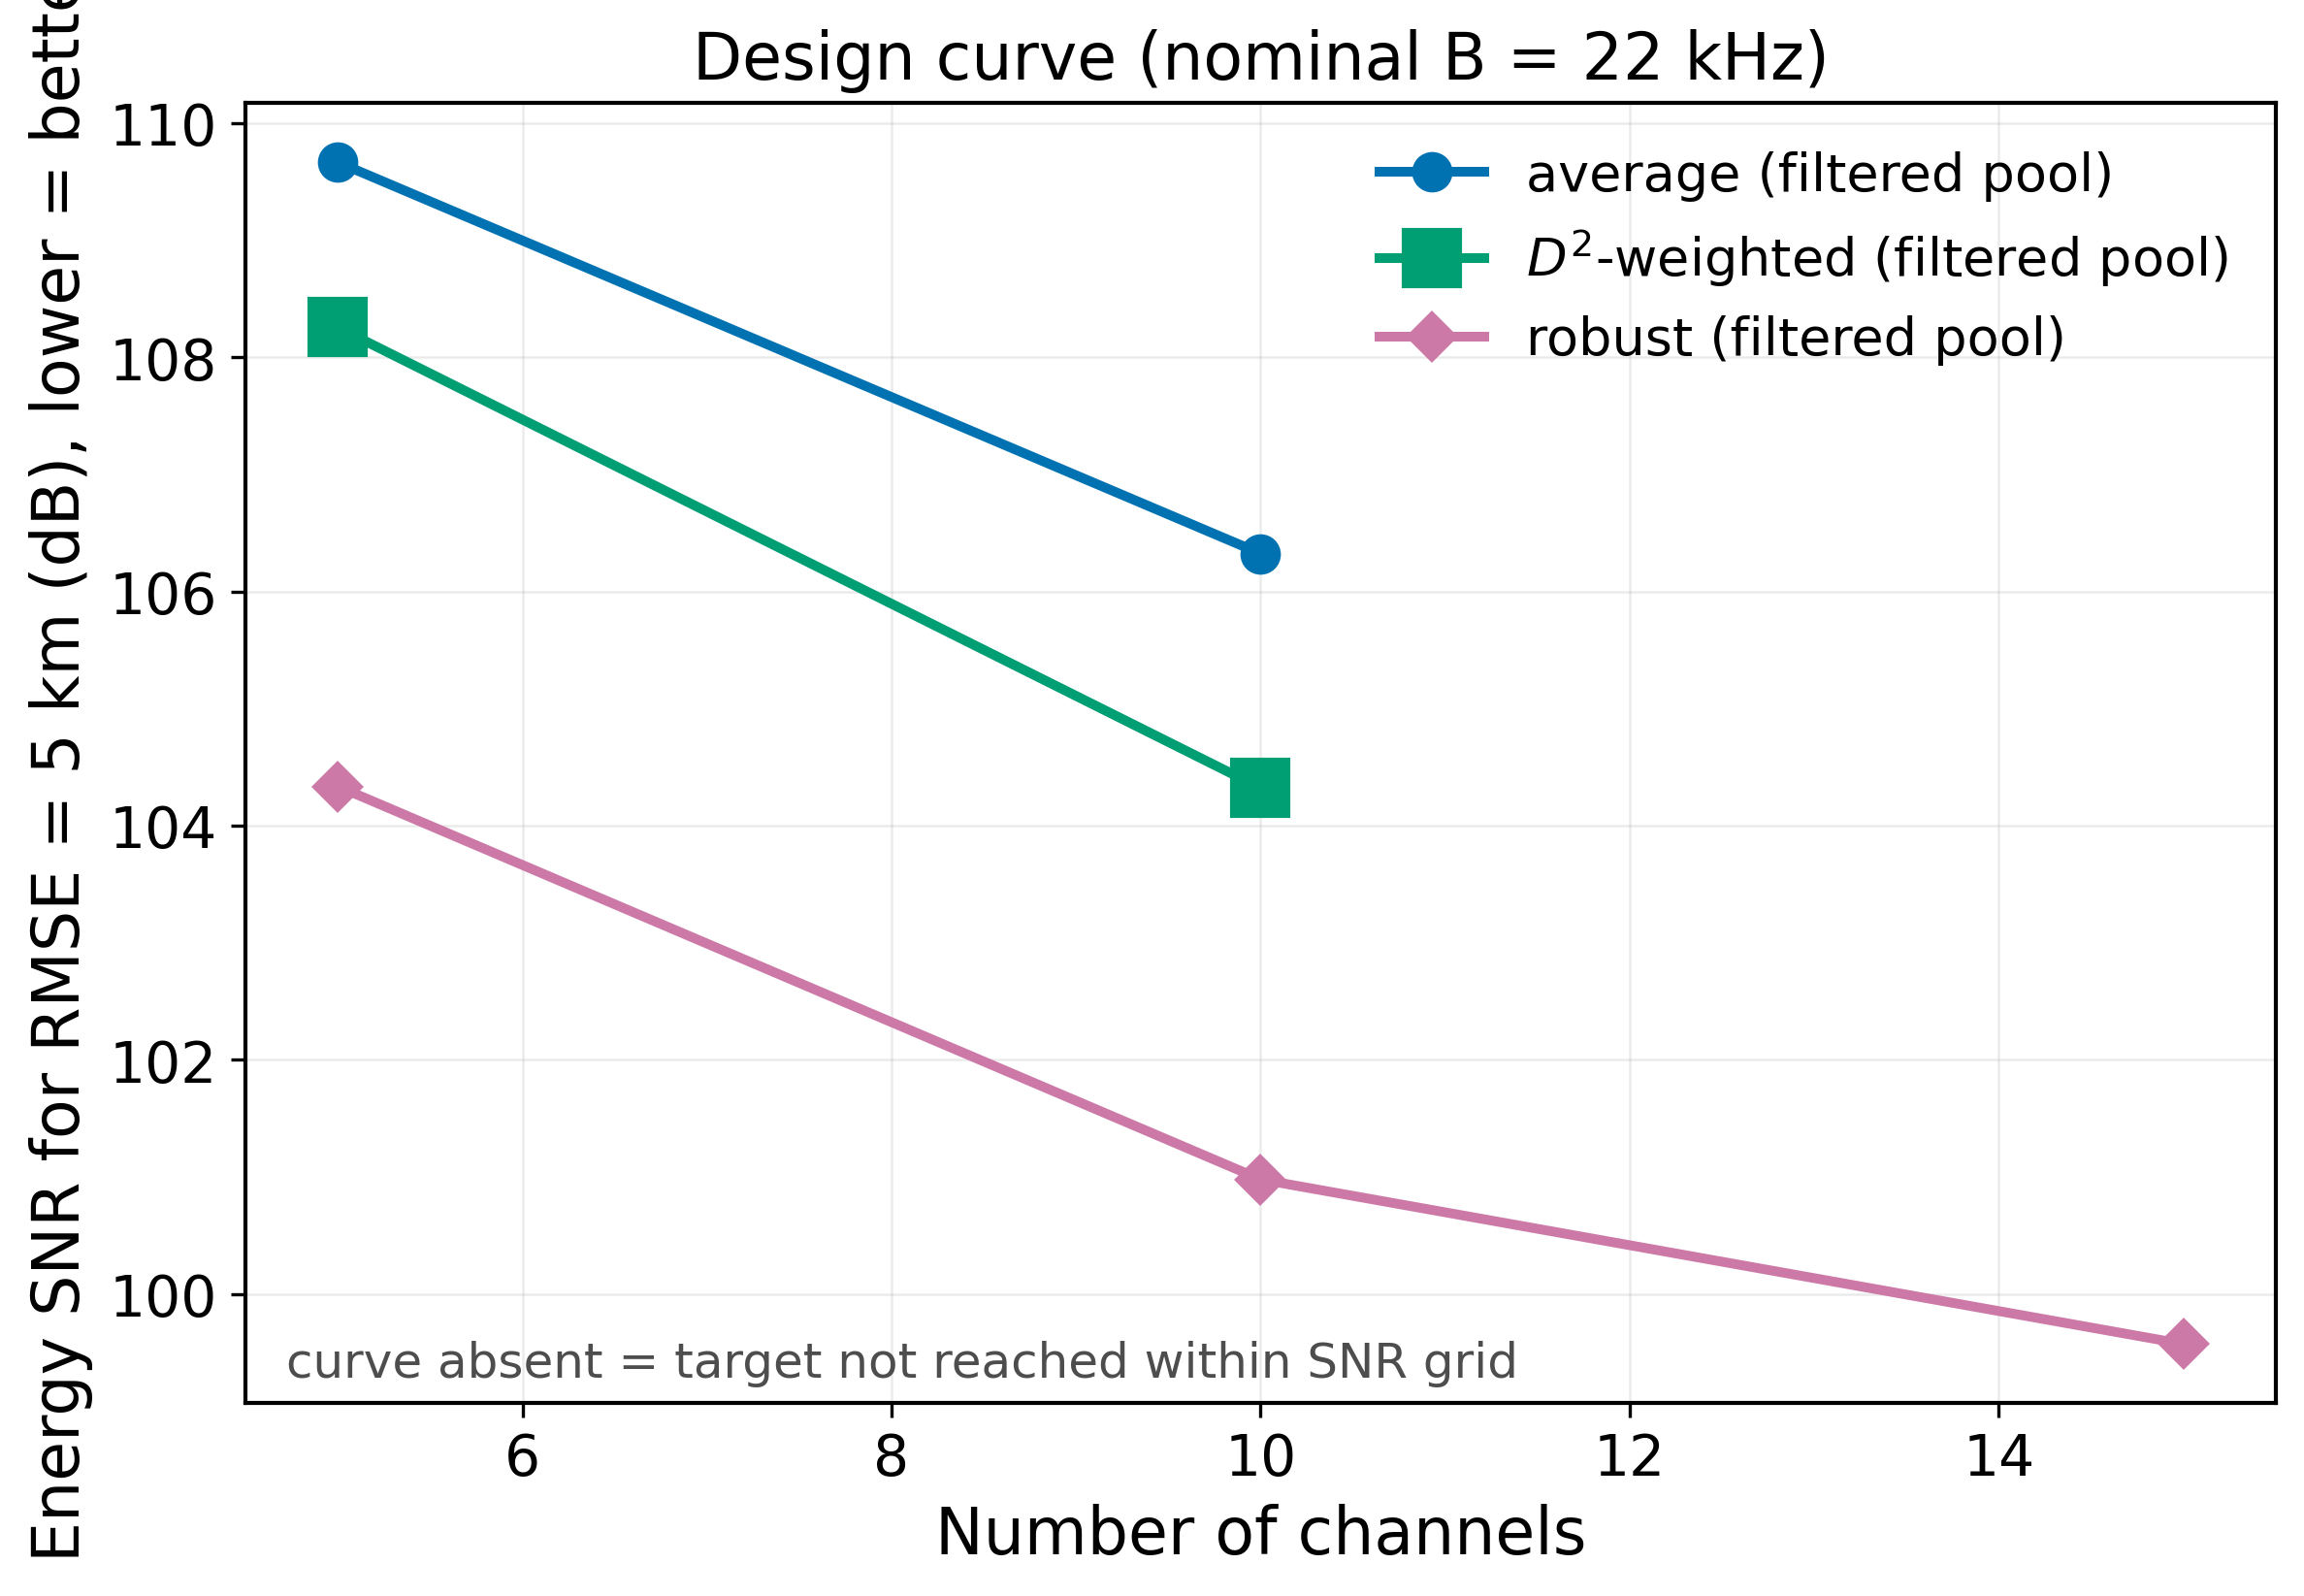
\includegraphics[width=\linewidth]{F4_db_gain_vs_channels.png}
\caption{Empirical design curve: mean per-component energy SNR required to
reach RMSE $=5$\,km versus channel count (lower is better) for the equispaced
GCC-PHAT run at nominal $B\approx22$\,kHz, using the filtered pool. The
missing 15-channel points for equal and $D^2$ fusion mean those methods did
not reach 5-km RMSE within the saved SNR range; the robust method did.}
\label{fig:design}
\end{figure}

\begin{figure}[t]
\centering
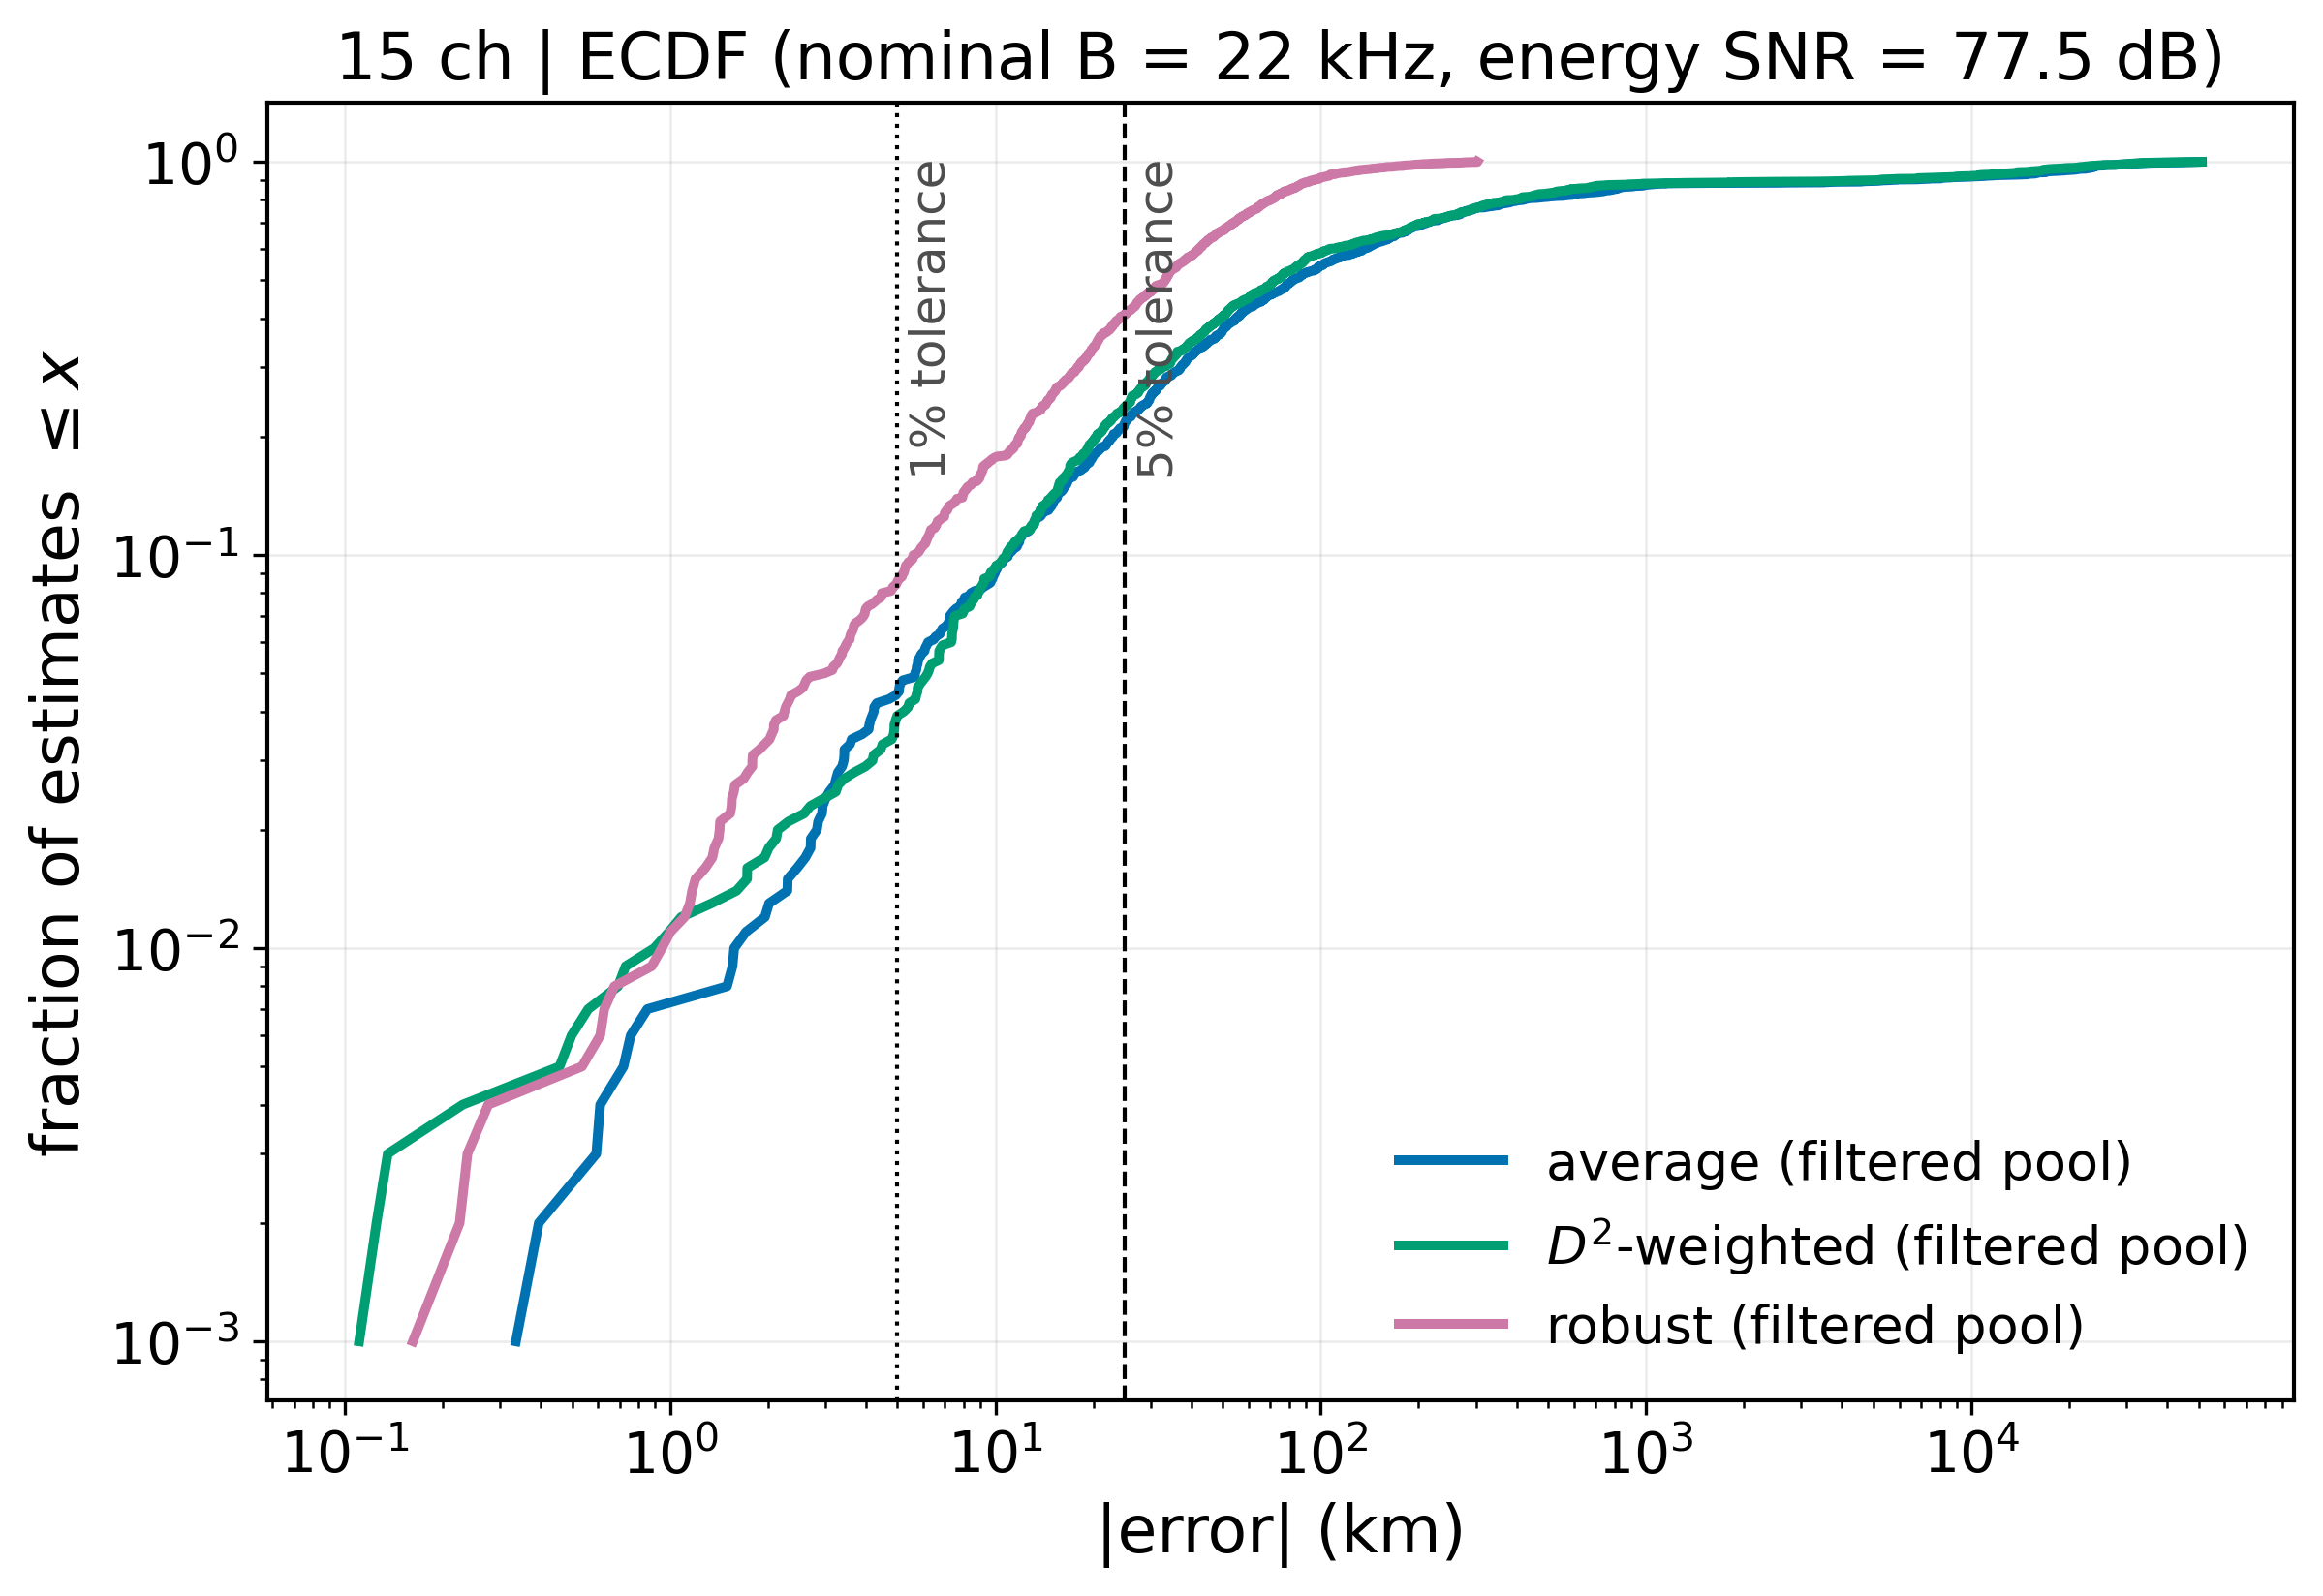
\includegraphics[width=0.9\linewidth]{F5_error_distributions.png}
\caption{ECDF of absolute range error for the 15-channel equispaced GCC-PHAT
run at nominal $B\approx22$\,kHz and energy SNR $77.48$\,dB. All curves use the
$\alpha=0.25$ filtered pool. Curves farther left and higher indicate a larger
fraction of smaller absolute errors; the robust pool has the lightest
large-error tail in this selected cell.}
\label{fig:ecdf}
\end{figure}

\section{Discussion and design rules}
\label{sec:discussion}
The results support a conditional, practical story: a broadband event can
provide precise timing, and a WDM comb supplies multiple pairwise delay
measurements, but the usable gain depends on whether the event is visible in
each channel, the dispersion distribution across the selected channels, and
the estimator's pair-level error pattern. A useful workflow is:
\begin{enumerate}
\item \textbf{Check cross-channel observability first.} The method is suitable
when a transient leaves a measurable, temporally identifiable signature in
several channels and the CD-versus-wavelength calibration is known. It does
not require identifying the event's physical mechanism, but it is not validated
for arbitrary waveforms or events absent from some channels.
\item \textbf{Inspect the pair-dispersion distribution.} A large
$D_{ij}^{\rm abs}$ maps a given delay error to a smaller distance error.
Equispaced layouts provide a graded distribution: continuous $D^2$ weighting
retains nonzero weights for weaker-dispersion pairs, while a hard threshold
removes them. The alternating band-edge layout creates a much more separated
low/high group, so soft $D^2$ weighting nearly reproduces hard selection.
\item \textbf{Start with all-pair $D^2$ and robust fusion, then compare with a
fixed hard threshold.} $D^2$ uses known geometry only; the robust rule adds
realization-specific residual rejection. The former is a simple marginal
variance heuristic; neither method accounts for the full pair covariance.
The robust method often helps in the saved equispaced runs, particularly for
GCC-PHAT outliers, but is not guaranteed to win and can fail if the pair
consensus is itself wrong.
\item \textbf{Choose the delay estimator using both variance and bias.}
Parabolic interpolation can be lower variance, especially at lower SNR, but
its peak-shape bias can dominate at high SNR. GCC-PHAT can reduce that bias at
some bandwidths, at the cost of sensitivity to weak/noisy spectral bins and
possible outlier peaks. The crossover is regime-dependent.
\item \textbf{Treat channel pairs as correlated measurements.} The number of
available pairs grows as $N(N-1)/2$, but this is not the number of independent
observations and does not imply a $1/\sqrt{N_{\rm pairs}}$ error law. Report
empirical RMSE and its bias/spread decomposition; use only a validated joint
covariance or waveform model for theoretical multichannel bounds.
\end{enumerate}

\textbf{Limitations and scope.} This is a simulation study of one class of
localized SOP perturbation. The event signature must be detectable across
channels; performance for every physical transient mechanism is not claimed.
The local PMD response is simulated over a 0.5-km section centered 500 km from
the receiver, while the remaining path contributes deterministic CD shifts but
no distributed PMD. Receiver effects, experimental channel imbalance, and
uncertainty in the dispersion calibration are not included. The noise model is
additive, white, and independent across channels/components. The empirical
fusion numbers are point estimates without paired confidence intervals; small
sub-dB differences should not be interpreted as statistically resolved. The
additive channel-timing covariance model is not adequate in every sweep cell,
and the held-out covariance GLS is a benchmark rather than a bound. Finally,
parabolic interpolation bias is measured but not corrected.

\section{Conclusion}
\label{sec:conclusion}
We derived and numerically checked a two-sensor effective-SNR CRB for the
relative delay of two noisy SOP records, then converted that per-pair timing
reference to distance through the integrated chromatic dispersion. The saved
Monte-Carlo results show that WDM channel diversity can reduce the SNR required
for a target range error, but the useful gain depends on how the wavelengths
populate the dispersion axis and how pair errors are fused. On the equispaced
grid, all-pair $D^2$ weighting is close to a hard-filtered equal average, while
robust all-pair fusion can provide additional empirical gains. On the
alternating band-edge grid, filtering removes a low-dispersion group whose
aggregate $D^2$ weight is almost negligible, so $D^2$ weighting and filtering
become nearly equivalent. Delay-estimator bias can dominate at high SNR, so
neither a single fusion rule nor a single delay estimator is uniformly best.
We do not claim that the fused result attains a universal combined CRB or that
every event waveform is suitable. Future work should add paired uncertainty
analysis, a joint waveform-level bound, experimental validation,
bias-corrected peak estimation, and channel-selection optimization.

\begin{thebibliography}{9}
\bibitem{taylor1993das} H.~F. Taylor and C.~E. Lee, ``Apparatus and method for
fiber optic intrusion sensing,'' U.S. Patent 5,194,847 (1993).
\bibitem{he2021das} Z.~He and Q.~Liu, ``Optical fiber distributed acoustic
sensors: A review,'' J. Lightwave Technol. \textbf{39}(12), 3671--3686 (2021),
doi:10.1109/JLT.2021.3059771.
\bibitem{sadler2006survey} B.~M. Sadler and R.~J. Kozick, ``A survey of time
delay estimation performance bounds,'' in \emph{Proc. Fourth IEEE Workshop on
Sensor Array and Multichannel Processing} (2006), pp.~282--288.
\bibitem{weiss1983} A.~J. Weiss and E.~Weinstein, ``Fundamental limitations in
passive time-delay estimation---Part I: Narrowband systems,'' IEEE Trans.
Acoust., Speech, Signal Process. \textbf{31}(2), 472--485 (1983).
\bibitem{knapp1976} C.~Knapp and G.~Carter, ``The generalized correlation method
for estimation of time delay,'' IEEE Trans. Acoust. Speech Signal Process.
\textbf{24}(4), 320--327 (1976).
\bibitem{gisin1992} N.~Gisin and J.~P. Pellaux, ``Polarization mode dispersion:
time versus frequency domains,'' Opt. Commun. \textbf{89}(2--4), 316--323 (1992).
\end{thebibliography}

\clearpage
\appendix
\section{Notation at a glance}
\begin{center}
\begin{tabular}{ll}
\toprule
Symbol & Meaning and units \\
\midrule
$Z$ & event range from receiver (km) \\
$N_s$, $C$ & samples per record; real SOP components ($C=2$) \\
$\sigma^2$, $N_0$ & discrete sample-noise variance; $N_0=\sigma^2dt$ \\
$\SNR_E$ & mean per-component energy SNR (linear ratio or dB) \\
$B_{\rm nom}$ & nominal Gaussian-envelope parameter (Hz) \\
$\beta$ & measured SOP RMS angular-frequency bandwidth (rad/s) \\
$D_{ij}^{\rm abs}$ & integrated CD magnitude (ps/km) between two carriers \\
$\tau_{ij}$, $\hat\tau_{ij}$ & true and estimated pair delay (s) \\
$\hat Z_{ij}$ & pair range estimate (km) \\
$\alpha$ & pair-selection threshold on $D^2/\max D^2$ \\
$N_p$ & available pair count, $N(N-1)/2$ \\
\bottomrule
\end{tabular}
\end{center}

\section{Delay-bound derivation and units}
\label{app:bound}
This appendix collects the derivation details behind the pairwise reference.
It is included to make the conventions auditable; it does not create a
multichannel bound by summing pair information.

\subsection{Deterministic known-waveform Fisher information}
For independent real components observed in additive Gaussian noise, the
log-likelihood, up to an additive constant, is
\begin{equation}
\ell(\tau)=-\frac{1}{2\sigma^2}\sum_{c=1}^C\sum_{n=0}^{N_s-1}
\left(x_c[n]-s_c(t_n-\tau)\right)^2.
\end{equation}
Differentiating with respect to delay and taking the expected squared score
gives
\begin{equation}
J_{\rm det}(\tau)=\frac{1}{\sigma^2}\sum_c\sum_n
\left|\frac{\partial s_c(t_n-\tau)}{\partial\tau}\right|^2
\simeq\frac{1}{\sigma^2dt}\sum_c\int
\left|\frac{\partial s_c(t-\tau)}{\partial\tau}\right|^2dt
=\frac{1}{N_0}\sum_c\int
\left|\frac{\partial s_c(t-\tau)}{\partial\tau}\right|^2dt,
\qquad N_0=\sigma^2dt.
\end{equation}
In continuous time, Parseval's theorem gives
\begin{equation}
\int\left|\frac{\partial s_c(t-\tau)}{\partial\tau}\right|^2dt
=\int(2\pi f)^2|S_c(f)|^2df
=E_c\beta_c^2,
\quad E_c=\int|s_c(t)|^2dt,
\quad \beta_c^2=\frac{\int(2\pi f)^2|S_c(f)|^2df}{E_c}.
\end{equation}
Thus $\CRB_{\rm det}(\tau)=1/J_{\rm det}$. In discrete records,
$E_c\simeq dt\sum_n s_c[n]^2$ and $N_0=\sigma^2dt$, so
$E_c/N_0=\sum_n s_c[n]^2/\sigma^2$. The factor $dt$ cancels in the energy
SNR, while $dt$ remains in the frequency grid used to calculate $\beta_c$.

\subsection{Two noisy observations and effective SNR}
For a pair of noisy channels, write the coherent signal-to-noise ratios at a
frequency as $\rho_i=S/N_i$ and $\rho_j=S/N_j$, where $S$ is the coherent
common-signal spectral power and $N_i,N_j$ are the channel noise spectral
powers. The two-sensor delay-information factor is
\begin{equation}
\rho_{\rm eff}=\frac{\rho_i\rho_j}{1+\rho_i+\rho_j}.
\end{equation}
If the two sensors have equal SNR $\rho$, this becomes
$\rho_{\rm eff}=\rho^2/(1+2\rho)$. At high SNR,
$\rho_{\rm eff}\simeq\rho/2$: uncertainty in both observations contributes,
so this stochastic pair bound is looser than the known-template deterministic
reference.

For $C$ independent components with the same per-component energy SNR
$\SNR_E$ and RMS bandwidth $\beta$, the deterministic and high-SNR effective
delay variances are, respectively,
\begin{equation}
\CRB_{\rm det}(\tau)=\frac{1}{C\SNR_E\beta^2},\qquad
\CRB_{\rm eff}(\tau)\simeq\frac{2}{C\SNR_E\beta^2}.
\end{equation}
For the simulated $C=2$, these are $1/(2\SNR_E\beta^2)$ and
$1/(\SNR_E\beta^2)$; the stochastic two-sensor standard deviation is larger
by $\sqrt2$ in this limit.

\subsection{Discrete spectra, endpoint weights, and distance units}
The discrete Fourier transform convention in the code is
$X[k]=\sum_{n=0}^{N_s-1}x[n]e^{-2\pi i kn/N_s}$. For real records, an
$r$FFT stores the nonnegative frequencies. A full two-sided sum is recovered
using
\begin{equation}
q_k=\begin{cases}
1,& k=0,\\
1,& k=N_s/2\quad(N_s\text{ even}),\\
2,&\text{all other stored }r\text{FFT bins}.
\end{cases}
\end{equation}
The Nyquist bin exists only for even $N_s$ and has no distinct negative
frequency partner. The mean-square bandwidth is therefore computed as
\begin{equation}
\beta^2=\frac{\sum_{k\in\mathcal K_r}q_k(2\pi f_k)^2
\sum_c|X_c[k]|^2}
{\sum_{k\in\mathcal K_r}q_k\sum_c|X_c[k]|^2}.
\end{equation}
In the effective-SNR Fisher information, $q_k$ weights each component's
frequency-bin information in the same manner. DC contributes no delay
information because $2\pi f_0=0$.

The dispersion integral has units ps/km when $D$ is in ps/(nm km) and
wavelength is in nm. Define the signed delay slope
$\Delta d_{ij}=10^{-12}\int_{\lambda_j}^{\lambda_i}D(\lambda)d\lambda$
in seconds/km. Then $\tau_{ij}=Z\Delta d_{ij}$ and
\begin{equation}
\sigma_{Z,ij}=\frac{\sigma_{\tau,ij}}{|\Delta d_{ij}|}
=\frac{10^{12}\sigma_{\tau,ij}}{D_{ij}^{\rm abs}}\quad[\mathrm{km}].
\end{equation}

\section{Pair covariance, GLS, and fusion}
\label{app:fusion}
For the additive channel-timing model, let $A$ be the signed incidence matrix
defined in Sec.~\ref{sec:crb}. Its covariance has entries
\begin{equation}
\operatorname{Cov}(e_{ij},e_{kl})=
\sum_{m=1}^{N}A_{(ij),m}A_{(kl),m}u_m.
\end{equation}
Disjoint pairs have zero covariance under this particular model; pairs sharing
a channel generally do not. For example,
$\operatorname{Cov}(e_{ij},e_{ik})=u_i$ when both signed differences use channel $i$ with a
positive sign. Reversing a pair orientation changes the corresponding signs.
This model is a useful illustration of correlation, but the measured
cross-correlation errors need not obey it exactly.

If $\Sigma_Z$ were known and the pair estimates unbiased, minimizing the
variance of a linear estimator $a^T\hat{\boldsymbol Z}$ subject to
$a^T\mathbf1=1$ yields, by a Lagrange multiplier,
\begin{equation}
a_{\rm GLS}=\frac{\Sigma_Z^{-1}\mathbf1}
{\mathbf1^T\Sigma_Z^{-1}\mathbf1},\qquad
\Var(a_{\rm GLS}^T\hat{\boldsymbol Z})=
\frac{1}{\mathbf1^T\Sigma_Z^{-1}\mathbf1}.
\end{equation}
This is a BLUE result under the assumed covariance and common-mean model. It
does not imply that an empirical sample covariance is a CRB, nor that its
weights correct estimator bias.

The robust pair weights in Eq.~\eqref{eq:robustweights} are also worth reading
as two factors. $D_{ij}^2$ encodes prior geometric sensitivity; $\psi(r_{ij})$
is a data-dependent inlier factor. The threshold rule in
Eq.~\eqref{eq:alphapool} is different: it sets a pair's weight exactly to zero
or leaves it in the pool before fusion. The F11 weight-share calculation
normalizes the deterministic $D^2$ weights by $\sum_{ij}D_{ij}^2$; it does
not measure a pair's independent information or the signed contribution of
its random error to a particular fused estimate.

\section{Monte-Carlo metrics and target-SNR interpolation}
\label{app:metrics}
Let $e_m=\hat Z_m-Z$ denote the error over $M$ realizations. The decomposition
used in the sweep is
\begin{equation}
\mathrm{MSE}=\frac1M\sum_m e_m^2
=\left(\frac1M\sum_m e_m\right)^2
+\frac1M\sum_m\left(e_m-\frac1M\sum_q e_q\right)^2
=\mathrm{bias}^2+\mathrm{std}^2.
\end{equation}
The empirical CDF shown in F5 is
$F_{|e|}(x)=M^{-1}\#\{m:|e_m|\le x\}$. At a true range of 500 km, 1\% and
5\% relative-error thresholds are 5 km and 25 km.

For target $R_*$, suppose two adjacent saved SNR points satisfy
$R_0>R_*$ and $R_1\le R_*$. The reported crossing is interpolated as
\begin{equation}
\SNR_* = \SNR_0+(\SNR_1-\SNR_0)
\frac{\log_{10}R_*-\log_{10}R_0}
{\log_{10}R_1-\log_{10}R_0}.
\end{equation}
If no saved RMSE point reaches $R_*$, the crossing is undefined; the design
curve leaves that method/channel-count point blank rather than extrapolating.
All such crossings and small dB savings in this draft are point estimates.

\end{document}
